\documentclass[12pt, oneside]{book}
\usepackage[utf8]{inputenc}
\usepackage[a4paper,top=2.5cm,bottom=2.5cm,left=3.5cm,right=2cm]{geometry}
\usepackage{graphicx}
\usepackage{float}
\usepackage{caption}
\usepackage{setspace}
\usepackage{array}
\usepackage{longtable}
\usepackage{hyperref} % Permite crear enlaces clicables
\usepackage[spanish]{babel} % Para que las etiquetas como "Referencias" salgan en español
\addto\captionsspanish{\renewcommand{\tablename}{Tabla}}
\addto\captionsspanish{\renewcommand{\listtablename}{Índice de tablas}}
\renewcommand{\arraystretch}{1.35}
\captionsetup{skip=10pt}
\setlength{\intextsep}{16pt}
\setlength{\textfloatsep}{18pt}
\setlength{\floatsep}{16pt}
% --- AQUÍ EMPIEZA EL CONTENIDO ---
\begin{document}


\thispagestyle{empty}

\begin{center}
\begin{figure}
\begin{center}

\includegraphics[height=4cm]{images/Logo_UNLP.jpg}
\end{center}
\end{figure}
\small

\vfill
\Large
\textbf{Evaluación del desempeño de modelos de Deep Learning en 
dispositivos móviles para el reconocimiento en tiempo real de enfermedades en plantas} \\ 


\vfill
\large
\textbf{Tesista:} Stefany Carolina Chávez David\\
\textbf{Director:} Federico Balaguer \\

\vfill
\large
Tesis presentada para obtener el grado de Magister en  \\
Ingeníera de Software\\
Facultad de Informática - Universidad Nacional de La Plata\\
La Plata, Argentina\\
2026

\end{center}




\tableofcontents
\chapter{Introducción}

Argentina destaca por estar entre los países exportadores agrícolas más importantes del mundo. Según el Banco Mundial, en 2021 el sector agroalimentario
representó aproximadamente el 15,7\% del Producto Interno Bruto (PIB) nacional y generó cerca del 10,6\% de los ingresos fiscales del país \cite{worldbank2024agricultura}. 
La amplia extensión de tierras agrícolas (aproximadamente el 47\% del territorio argentino) sustenta cultivos y producciones que abastecen 
tanto el mercado interno como la exportación \cite{usda2024argentina}. Además, productos como la soja, el maíz y el trigo representan alrededor del 36\% de los ingresos
por exportaciones del país. Al considerar de manera conjunta los productos primarios y las manufacturas de origen agropecuario, el sector alcanza 
aproximadamente el 60\% de las exportaciones totales de Argentina \cite{millermagazine2024argentina}, lo que consolida al sector agrícola como un actor clave para la estabilidad 
económica, la generación de divisas y el sostenimiento del empleo rural.

Las enfermedades en plantas y las plagas constituyen un riesgo permanente   
para los cultivos; en Argentina, los sistemas productivos enfrentan una amplia variedad de enfermedades fúngicas, bacterianas y virales que generan
pérdidas significativas y requieren monitoreo constante para preservar los rendimientos y la calidad de producción \cite{aapresid2024maiz}. La detección tradicional de 
enfermedades se basa en la observación visual en campo y en análisis de laboratorio realizados por organismos como el Servicio Nacional de Sanidad y
Calidad Agroalimentaria (SENASA) \cite{argentina2024laboratorio}.  Estas técnicas permiten identificar síntomas visuales característicos en las hojas, tales como lesiones
necróticas, alteraciones en la coloración y deterioro del tejido vegetal, así como confirmar la presencia de patógenos mediante métodos moleculares,
contribuyendo al manejo integrado de plagas y enfermedades. En paralelo, en los últimos años se han desarrollado herramientas tecnológicas 
orientadas a asistir y automatizar el monitoreo sanitario de los cultivos, incluyendo el uso de sensores, drones y sistemas de análisis de imágenes.
Estas soluciones buscan ampliar la cobertura del monitoreo y reducir la dependencia exclusiva de la inspección manual. Sin embargo, en zonas rurales 
o remotas, donde la conectividad es intermitente o inexistente, el acceso oportuno a plataformas digitales o a sistemas que dependen de infraestructura
externa resulta limitado.

En las últimas décadas, el aumento de la capacidad de cómputo, el acceso a grandes conjuntos de datos y el desarrollo de algoritmos avanzados han 
impulsado la adopción de la Inteligencia Artificial (IA) en una amplia variedad de dominios \cite{dhar2019ondevice}. En el sector agrícola, la creciente demanda de 
agricultura de precisión ha promovido la exploración de tecnologías basadas en IA para mejorar el rendimiento de los cultivos y optimizar el 
monitoreo de enfermedades \cite{ahmed2021mobile,johannes2017automatic,Niaz2025Efficient}. Uno de los enfoques más prometedores es el diagnóstico automatizado de enfermedades foliares, que emplea 
técnicas de visión por computadora, procesamiento de imágenes y algoritmos de aprendizaje automático (Machine Learning, ML) y aprendizaje profundo (Deep Learning, DL) para identificar 
patologías a partir de imágenes \cite{agronomy13040961}. Esta capacidad, sumada a la democratización de la tecnología mediante el uso de dispositivos móviles, 
permite el desarrollo de herramientas accesibles como apoyo en el proceso de inspección visual, sin necesidad de especialistas ni infraestructura 
compleja.

Muchos estudios en los que se implementan modelos de aprendizaje automático y aprendizaje profundo en dispositivos móviles dependen del procesamiento en 
la nube \cite{ahmed2021mobile,Tembhurne2023}, lo que introduce limitaciones como latencia, dependencia de la conectividad y riesgos de privacidad asociados al envío de 
información a servidores externos \cite{xiao2025understanding}. En contraste, la inferencia directa en el dispositivo (on-device), mediante la ejecución del modelo en 
el hardware del teléfono, permite procesar los datos localmente, reduciendo la latencia, preservando la privacidad y habilitando el funcionamiento 
sin conexión \cite{dhar2019ondevice}. Además, al prescindir de recursos en la nube, se disminuyen los costos operativos y se mejora la accesibilidad 
de la solución.

A pesar de estos beneficios, la implementación de modelos de aprendizaje profundo en dispositivos móviles enfrenta retos técnicos significativos.
Los dispositivos móviles tienen recursos limitados de memoria, procesamiento y energía, lo que restringe la complejidad de los modelos que pueden 
ejecutarse sin comprometer la eficiencia. Por eso, es fundamental encontrar un equilibrio adecuado entre precisión del modelo, consumo de recursos
(latencia, energía, memoria) y tamaño de la aplicación.

En este escenario, las arquitecturas ligeras como MobileNet y EfficientNet han demostrado un rendimiento competitivo en tareas de clasificación bajo
restricciones de hardware \cite{zainab2025plant,geetharamani2019identification,subramaniam2026comparative}. Sin embargo, gran parte de los trabajos revisados se concentra principalmente en métricas de precisión del modelo, mientras que son 
más limitados los estudios que analizan de manera comparativa y sistemática el desempeño conjunto de precisión y eficiencia computacional directamente
en dispositivos móviles reales, bajo condiciones controladas y medibles.

Por lo tanto, se vuelve relevante desarrollar un estudio que evalúe comparativamente estas arquitecturas en un entorno de inferencia en el dispositivo, utilizando métricas 
integradas de desempeño (exactitud, sensibilidad y F1-score) junto con métricas de eficiencia (latencia de inferencia, uso de CPU, consumo de memoria, 
energía y tamaño del modelo). Este análisis permitirá determinar la viabilidad técnica real de soluciones basadas en aprendizaje profundo ejecutadas 
localmente en dispositivos móviles, aportando evidencia empírica sobre su aplicabilidad en escenarios rurales con conectividad limitada y 
contribuyendo al diseño de sistemas agrícolas inteligentes con enfoque local.

\section{Objetivos}

\subsection{Objetivo general}

Evaluar la viabilidad técnica del reconocimiento de enfermedades en plantas mediante arquitecturas ligeras de aprendizaje profundo
ejecutadas en dispositivos móviles sin dependencia de conectividad a internet, analizando su desempeño en términos de precisión de
clasificación, eficiencia de ejecución y uso de recursos computacionales.

\subsection{Objetivos específicos}

Para alcanzar este objetivo general, se plantean los siguientes objetivos específicos:

\begin{itemize}
    \item Preparar y preprocesar el conjunto de datos PlantVillage para el entrenamiento, validación y prueba de modelos de clasificación de 
    enfermedades en hojas de plantas.
    \item Implementar y entrenar arquitecturas ligeras de aprendizaje profundo, específicamente MobileNetV3 Small y EfficientNetV2B0, 
    utilizando técnicas de transferencia de aprendizaje y ajuste fino.
    \item Convertir los modelos entrenados a un formato compatible con dispositivos Android mediante TensorFlow Lite, considerando una 
    representación optimizada para su ejecución en el dispositivo.
    \item Desarrollar una aplicación móvil prototipo que permita ejecutar inferencias localmente sobre imágenes de hojas, sin dependencia de 
    servicios externos ni conectividad a internet.
    \item Evaluar comparativamente los modelos en dispositivos móviles con distintas capacidades de hardware, considerando métricas de 
    clasificación, latencia, memoria, consumo energético, temperatura y tamaño del modelo.
    \item Analizar el comportamiento de los modelos frente a imágenes capturadas en condiciones menos controladas que PlantVillage, 
    incluyendo fondos complejos, variaciones de iluminación e imágenes fuera del dominio esperado.
\end{itemize}

\chapter{Marco Teórico}

En esta sección se presentan los conceptos fundamentales relacionados con el reconocimiento de imagenes enfocado al 
diagnóstico de enfermedades foliares utilizando arquitecturas ligeras de aprendizaje profundo en dispositivos móviles.
Se abordan temas  los modelos de aprendizaje profundo, transfer learning y los desafíos asociados a la implementación
en dispositivos móviles.



\section{Redes neuronales convolucionales para clasificación de imágenes}
Las redes neuronales convulucionales (CNN) son un tipo de arquitectura de aprendizaje profundo que se ha vuelto muy popular en los 
ultimos años, especialemente en tareas de clasificación de imágenes. Estan diseñadas para reconocer objetos usando capas
que incluyen la convolución, la activación y el pooling. Estas capas permiten a las CNN aprender características jerárquicas de
las imágenes, desde bordes y texturas simples en las primeras capas hasta patrones más complejos en las capas posteriores.
Ademas estas capas trabajan juntas usando backprogation para adaptar y mejorar la red. El objetivo principal de esta las CNN es 
crear una red más extensa con menos parámetros \cite{agronomy13040961}.


\subsection{Transfer Learning y ajuste fino}
Las redes neuronales convolucionales (CNN) han demostrado un rendimiento sobresaliente en tareas de 
clasificación de imágenes, pero su entrenamiento desde cero requiere grandes cantidades de datos y recursos computacionales.
El transfer learning es una técnica que permite aprovechar el conocimiento adquirido por un modelo preentrenado en una tarea relacionada 
para mejorar el rendimiento en una nueva tarea con menos datos. En este enfoque, se utiliza un modelo preentrenado 
como punto de partida y se ajusta (fine-tuning) para adaptarlo a la nueva tarea específica, lo que puede resultar en una mejora
significativa en la precisión del modelo con un menor esfuerzo de entrenamiento.

La tecnica de transfer learning se ha vuelto especialmente relevante en el contexto de dispositivos móviles, donde las limitaciones
de recursos hacen que el entrenamiento desde cero sea impráctico. Hay una manera de acelerar el tiempo de entrenamiento, previniendo el 
overfitting, mejorando la interpretabilidad del modelo, reduciendo los requermientos de memoria y optimizando la eficiencia es utilizar
la tecnica de congelado de capas (layer freezing). Esta técnica consiste en mantener fijas las capas iniciales del modelo preentrenado,
ue suelen aprender características generales de las imágenes, y solo ajustar las capas finales, que se encargan de la
clasificación específica de la nueva tarea. Esto permite aprovechar el conocimiento general del modelo preentrenado mientras
se adapta a las particularidades de la nueva tarea con un menor riesgo de sobreajuste y una reducción significativa en el 
tiempo de entrenamiento \cite{zainab2025plant}.




\section{Arquitecturas ligeras para dispositivos móviles}

\section{Metodos de despligue}
Para hablar de la inferencia de modelos de inteligencias artificial en dispositivos móviles, es importante entender los conceptos de
inferencia en la nube e inferencia local. El paradigma tradicional de inferencia en la nube consisten en recolactar la informacion requerida
para la inferencia a nivel dispositivo El dispositivo se conecta a un servidor en la nube a traves de la red. Luego los modelos de inteligencia 
artificial operando en los servidores ejecutan la inferencia sobre la data y envian el resultado al dispositivo \cite{li2025empirical}.  

Los sitemas basados en la nube tienen acceso casi que a recursos ilimitados, unicamente limtados por el costo de los recursos utilizados, lo que los
hace ideales para escenarios de complejos de actividades de alto consumo de recursos como almacenamiento de data, procesamiento de data, 
entrenamiento de modelos, etc. Sin embargo, la inferencia en la nube tiene limitaciones que se vuelven mas promientes a medida IA constanteme se 
esta transformando en un factor clave en la vida cotidiana, especiamente den las aplicaciones móviles.\cite{dhar2019ondevice}. A continuacion se presentan algunas de las limitaciones mas importantes de la inferencia en la nube:
algunas de las desvantajas de la inferencia en la nube incluyen:

\begin{description}
    \item[Privacidad y seguridad:] La segurdidad es una de las preocupaciones mas importantes, ya que la data del usuario debe ser enviada a
servidores externos para su procesamiento y almacenamiento, lo que puede exponer la información a riesgos de seguridad y privacidad.
    \item[Latencia:] Esta es la descripción detallada del segundo punto.
\end{description}

Por otro lado la inferencia local, también conocida como inferencia en el dispositivo (on-device), se refiere a la ejecución de modelos 
de inteligencia artificial directamente en el hardware del dispositivo móvil, sin necesidad de enviar datos a servidores externos \cite{dhar2019ondevice}. Este enfoque tiene varias ventajas, como la reducción de la latencia, 
la mejora de la privacidad y la capacidad de funcionar sin conexión a internet lo que garantiza respuestas inmediatas y una mejora significativa
en la privacidad y seguridad de las aplicaciones. Sin embargo, también presenta desafíos técnicos
significativos debido a las limitaciones de recursos de los dispositivos móviles, como la memoria, el procesamiento y el consumo energético.
    
\subsection{Dispositivos edge}
Para enteder lo que implica la inferecias en el dispositivo se vuelve imperativo de definir lo que es un dispositvo edge. este se puede definir como
definir como aquel cuyos recursos de computación, memoria y energía son limitados y no pueden aumentarse ni disminuirse fácilmente ya sea por factor 
de forma o costo. dentro de esta categoría se encuentran los dispositivos móviles, como teléfonos inteligentes y tabletas,
así como también dispositivos IoT (Internet de las cosas)y otros dispositivos embebidos.

El hardware de los dispositivos edge se encuentra como la base de sus limitaciones. Inclusive es una linea de investigacion con el objetivo de 
desarrollar hardware especializado para mejorar el rendimiento de la inferencia en el dispositivo, como los procesadores de inteligencia
artificial (AI accelerators) y las unidades de procesamiento gráfico (GPUs) optimizadas para tareas de aprendizaje profundo. Sin embargo, 
es un proceso es un proceso costoso que requiere una gran inversión de capital para construir laboratorios e instalaciones de fabricación, y suele implicar
largos plazos de tiempo para su desarrollo.



\subsection{TensorFlow Lite, LiteRT y cuantización}
Todos los algoritmos de aprendizaje automático dependen de operaciones clave como la multiplicación-acumulación o Multiply-Add
en el caso de las redes neuronales. Las bibliotecas que soportan estas operaciones constituyen la interfaz que separa el hardware de 
los algoritmos de aprendizaje. Esta separación permite el desarrollo de algoritmos que no dependen de ninguna arquitectura de hardware específica.

Esta separación entre el software y el hardware es fundamental para la flexibilidad en la inteligencia artificial,
ya que permite que un mismo modelo pueda ejecutarse en diferentes dispositivos sin necesidad de ser rediseñado desde cero.

\section{Desafios tecnicos en la implementación de modelos de aprendizaje profundo en dispositivos móviles}

\subsection{Tiempo de procesamiento}
El tiempo de respuesta suele estar entre los factores más críticos para la usabilidad de cualquier aplicación en el dispositivo (on-device). 
Las dos medidas comúnmente utilizadas son el rendimiento (throughput) y la latencia. El rendimiento se mide como la tasa a la que se procesan los datos de 
entrada. Para maximizar el rendimiento, es común agrupar las entradas en lotes (batches), lo que resulta en una mayor utilización.
Sin embargo, realizar esta medición conlleva un tiempo de espera adicional para agregar los datos en dichos lotes. 
Por tanto, para casos de uso críticos en tiempo, la latencia es la medida utilizada con mayor frecuencia.

 \subsection{Memoria}
La memoria de un dispositivo proporciona un acceso inmediato a los datos en comparación con otros componentes de almacenamiento. 
Sin embargo, esta velocidad de acceso tiene costos más elevados. Por razones de costo, la mayoría de los dispositivos edge están diseñados con una memoria 
limitada. Como tal, la huella de memoria (memory footprint) de las aplicaciones edge suele estar adaptada para un dispositivo objetivo específico.

Los algoritmos de aprendizaje automático avanzados a menudo consumen una cantidad significativa de memoria durante la construcción del modelo,
debido al almacenamiento de los parámetros del modelo, variables auxiliares, etc. Por ejemplo, incluso modelos de clasificación de imágenes relativamente 
simples como ResNet-50 pueden ocupar megabytes de espacio en memoria

\subsection{Consumo energético}
El consumo de energía es otro factor crucial para la ejecución de modelos en dispositivos móviles. Una solución energéticamente eficiente puede prolongar 
la vida útil de la batería y reducir los costos de mantenimiento. La potencia del sistema, comúnmente estudiada en el desarrollo de hardware, 
es la relación entre el consumo de energía y el lapso de tiempo para una tarea determinada. 
Vincular el consumo de energía de una aplicación particular impulsada por IA para un dispositivo específico depende conjuntamente de una
serie de variables como el tiempo de ejecución, la memoria, etc. Capturar estas dependencias casi nunca es determinista.
Por ello, la mayoría de las investigaciones existentes estiman el uso de potencia/energía a través de una función sustituta (surrogate function)
que típicamente depende de la memoria y el tiempo de ejecución de una aplicación.



\input{state_art.tex}
\chapter{Metodología}










En este capítulo se describe la metodología utilizada para el entrenamiento, integración y evaluación de los modelos 
de deep learning orientados a la detección de enfermedades en hojas de plantas mediante una aplicación móvil.
El objetivo metodológico principal fue construir un flujo experimental que permitiera comparar dos arquitecturas diferentes 
de redes neuronales convolucionales, considerando no solo su desempeño predictivo, sino también su viabilidad de ejecución
en dispositivos móviles con recursos limitados. \\
La investigación se estructuró en distintas etapas: selección y preparación del conjunto de datos, 
entrenamiento de modelos de clasificación de imágenes, conversión de los modelos a un formato compatible con dispositivos Android, 
diseño de la interfaz de usuario para la aplicación móvil, desarrollo de la aplicación, integración de los modelos en la aplicación
móvil y evaluación experimental en condiciones controladas y reales. Esta metodologìa permitió analizar el comportamiento de los
modelos tanto en el entorno de desarrollo como en el dispositivo objetivo, manteniendo trazabilidad sobre las decisiones tomadas 
durante el proceso.



\section{Conjunto de datos}

Para el entrenamiento de los modelos se utilizó el conjunto de datos público PlantVillage \cite{DBLP:journals/corr/HughesS15},
ampliamente empleado en investigaciones relacionadas con la detección automática de enfermedades en plantas \cite{tembhurne2023plant24}. Este conjunto de datos
incluye 54.309 imágenes organizadas en 38 clases, correspondientes a hojas sanas y enfermas de 14 cultivos, manzana, arándano, cereza,
maíz, uva, naranja, melocotón, pimiento, patata, frambuesa, soja, calabaza, fresa y tomate. Se caracteriza por contar
con imágenes bien etiquetadas y de alta calidad, lo que permite construir un escenario de clasificación multiclase para evaluar el
desempeño de los modelos en un problema representativo a nivel investigativo.

En este estudio se utilizó el conjunto completo de cultivos disponibles. La selección de PlantVillage se fundamentó en su amplio uso
en la literatura científica, lo que favorece la comparabilidad y reproducibilidad de los resultados. Además, el conjunto de datos
incluye cultivos de alta relevancia productiva en Argentina, como soja y maíz. Dado que el objetivo de la investigación es evaluar la
viabilidad técnica y el desempeño en dispositivo móvil de arquitecturas ligeras de aprendizaje profundo, el enfoque adoptado es
independiente del cultivo particular y puede extenderse metodológicamente a otros contextos agrícolas.

En la figura \ref{fig:plantvillage_examples} se presentan algunos ejemplos de imágenes pertenecientes al conjunto de datos. Estas
muestras permiten observar el tipo de entrada visual utilizada durante el entrenamiento, así como parte de la variedad de cultivos y enfermedades
incluidas en el problema de clasificación.

\begin{figure}[H]
    \centering
    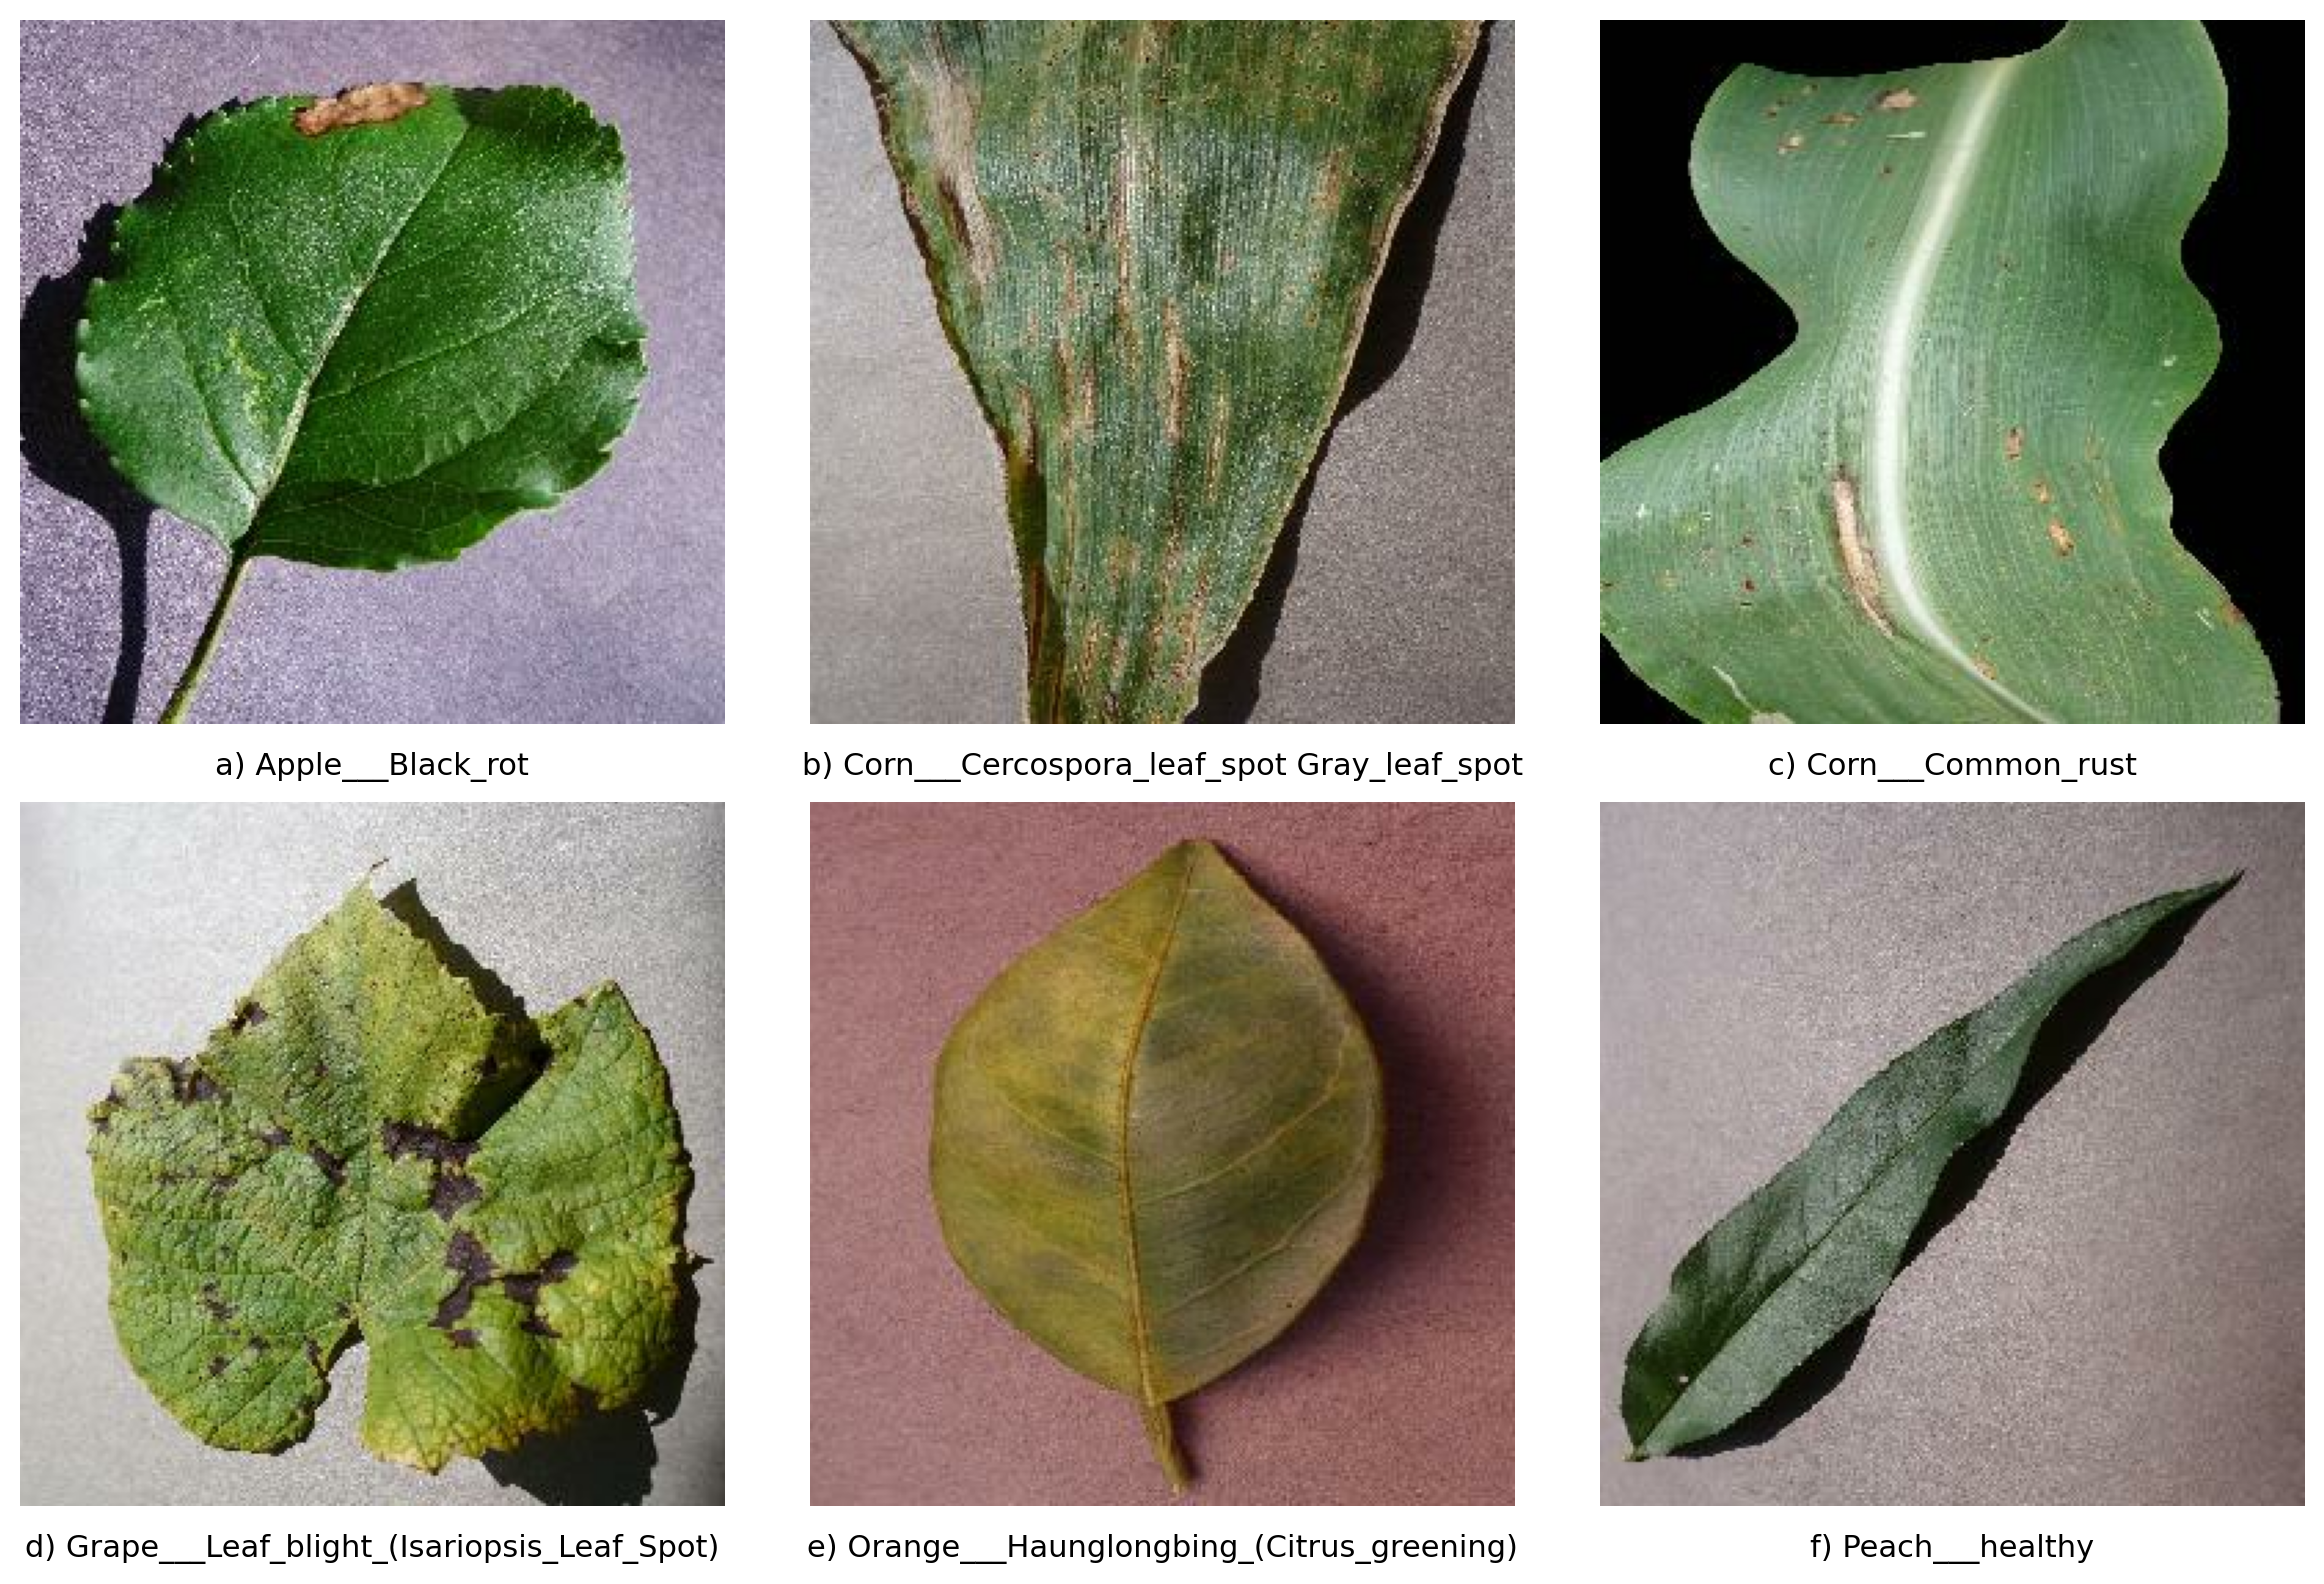
\includegraphics[width=1\textwidth]{images/ejemplos_plant_village.png}
    \caption{Ejemplos de imágenes del conjunto de datos PlantVillage: a) manzana con podredumbre negra, b) maíz con mancha foliar por Cercospora y mancha gris, c) maíz con roya común, d) uva con tizón foliar por Isariopsis, e) naranja con Huanglongbing o enverdecimiento de los cítricos, y f) durazno saludable.}
    \label{fig:plantvillage_examples}
\end{figure}

La distribución de imágenes por clase se puede observar en la figura \ref{fig:dataset_distribution}. Esta distribución permite
identificar la cantidad de ejemplos disponibles para cada categoría y ayuda a interpretar el comportamiento de los modelos durante
la evaluación, especialmente en un escenario donde se comparan clases de distintos cultivos y enfermedades.

\begin{figure}[H]
    \centering
    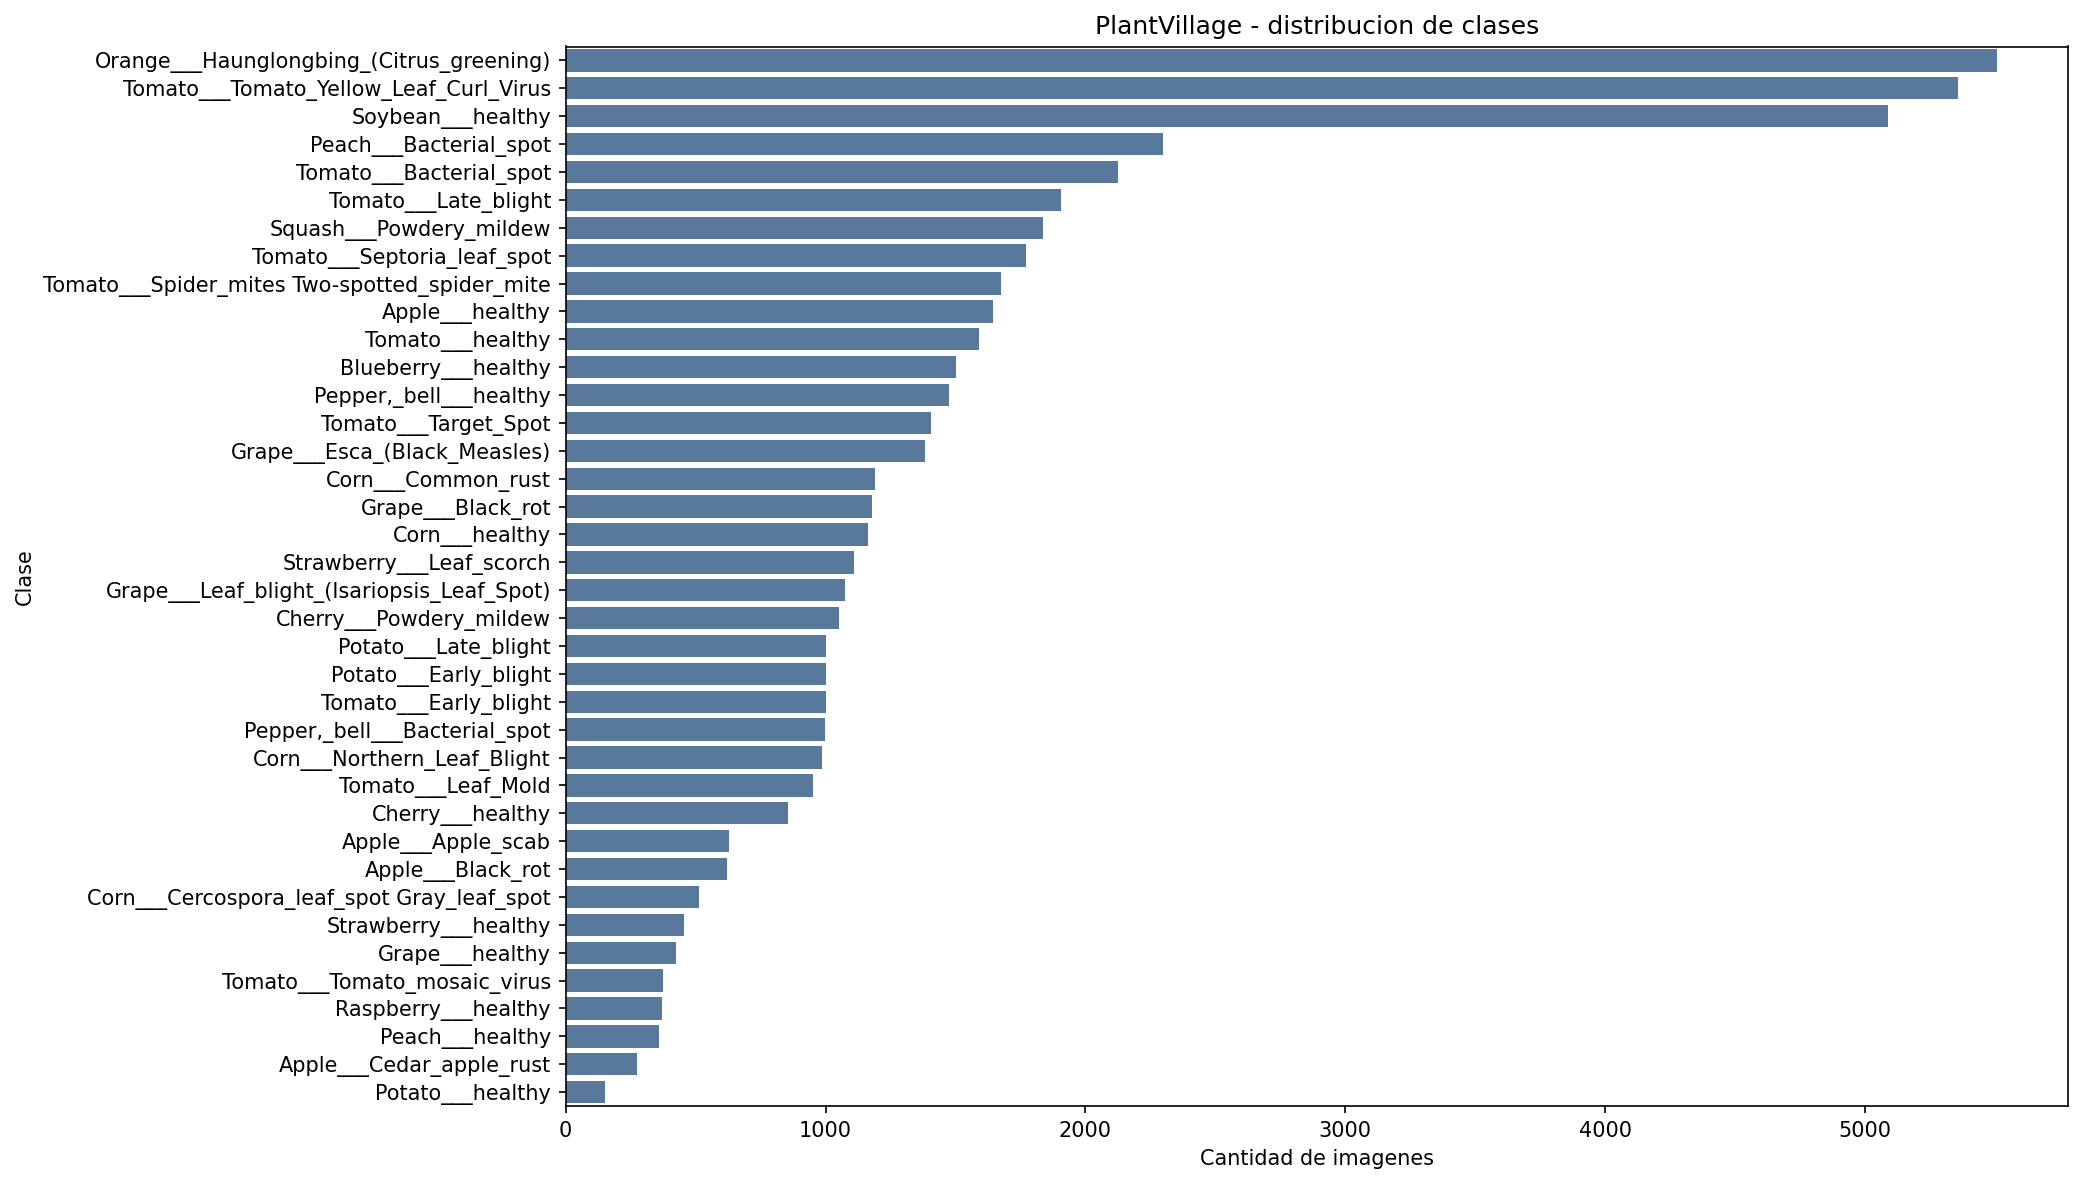
\includegraphics[width=1\textwidth]{images/dataset_distribution.png}
    \caption{Distribución del conjunto de datos PlantVillage por clase.}
    \label{fig:dataset_distribution}
\end{figure}

En la tabla \ref{tab:plantvillage_classes} se detallan las clases del conjunto de datos utilizadas en el entrenamiento, incluyendo
el cultivo, la enfermedad y el estado de salud de las plantas. Esta información es especialmente importante porque ayuda a comprender
la diversidad de casos que los modelos deben aprender a clasificar.


\begin{longtable}{>{\raggedright\arraybackslash}p{4.8cm}
                  >{\raggedright\arraybackslash}p{2.3cm}
                  >{\raggedright\arraybackslash}p{4.5cm}
                  >{\raggedright\arraybackslash}p{1.8cm}}
\caption{Clases del conjunto de datos PlantVillage utilizadas en el entrenamiento.}
\label{tab:plantvillage_classes}\\
\hline
\textbf{Clase} & \textbf{Cultivo} & \textbf{Enfermedad} & \textbf{Estado} \\
\hline
\endfirsthead
\hline
\textbf{Clase} & \textbf{Cultivo} & \textbf{Enfermedad} & \textbf{Estado} \\
\hline
\endhead
\path{Apple___Apple_scab} & Manzana & Sarna del manzano & Enferma \\
\path{Apple___Black_rot} & Manzana & Podredumbre negra & Enferma \\
\path{Apple___Cedar_apple_rust} & Manzana & Roya del cedro del manzano & Enferma \\
\path{Apple___healthy} & Manzana & Saludable & Saludable \\
\path{Blueberry___healthy} & Arándano & Saludable & Saludable \\
\path{Cherry___healthy} & Cereza & Saludable & Saludable \\
\path{Cherry___Powdery_mildew} & Cereza & Oídio & Enferma \\
\path{Corn___Cercospora_leaf_spot Gray_leaf_spot} & Maíz & Mancha foliar por Cercospora y mancha gris & Enferma \\
\path{Corn___Common_rust} & Maíz & Roya común & Enferma \\
\path{Corn___healthy} & Maíz & Saludable & Saludable \\
\path{Corn___Northern_Leaf_Blight} & Maíz & Tizón foliar del norte & Enferma \\
\path{Grape___Black_rot} & Uva & Podredumbre negra & Enferma \\
\path{Grape___Esca_(Black_Measles)} & Uva & Esca o sarampión negro & Enferma \\
\path{Grape___healthy} & Uva & Saludable & Saludable \\
\path{Grape___Leaf_blight_(Isariopsis_Leaf_Spot)} & Uva & Tizón foliar por Isariopsis & Enferma \\
\path{Orange___Haunglongbing_(Citrus_greening)} & Naranja & Huanglongbing o enverdecimiento de los cítricos & Enferma \\
\path{Peach___Bacterial_spot} & Durazno & Mancha bacteriana & Enferma \\
\path{Peach___healthy} & Durazno & Saludable & Saludable \\
\path{Pepper,_bell___Bacterial_spot} & Pimiento morrón & Mancha bacteriana & Enferma \\
\path{Pepper,_bell___healthy} & Pimiento morrón & Saludable & Saludable \\
\path{Potato___Early_blight} & Papa & Tizón temprano & Enferma \\
\path{Potato___healthy} & Papa & Saludable & Saludable \\
\path{Potato___Late_blight} & Papa & Tizón tardío & Enferma \\
\path{Raspberry___healthy} & Frambuesa & Saludable & Saludable \\
\path{Soybean___healthy} & Soja & Saludable & Saludable \\
\path{Squash___Powdery_mildew} & Calabaza & Oídio & Enferma \\
\path{Strawberry___healthy} & Frutilla & Saludable & Saludable \\
\path{Strawberry___Leaf_scorch} & Frutilla & Quemadura foliar & Enferma \\
\path{Tomato___Bacterial_spot} & Tomate & Mancha bacteriana & Enferma \\
\path{Tomato___Early_blight} & Tomate & Tizón temprano & Enferma \\
\path{Tomato___healthy} & Tomate & Saludable & Saludable \\
\path{Tomato___Late_blight} & Tomate & Tizón tardío & Enferma \\
\path{Tomato___Leaf_Mold} & Tomate & Moho foliar & Enferma \\
\path{Tomato___Septoria_leaf_spot} & Tomate & Mancha foliar por Septoria & Enferma \\
\path{Tomato___Spider_mites Two-spotted_spider_mite} & Tomate & Ácaro de dos manchas & Enferma \\
\path{Tomato___Target_Spot} & Tomate & Mancha objetivo & Enferma \\
\path{Tomato___Tomato_mosaic_virus} & Tomate & Virus del mosaico del tomate & Enferma \\
\path{Tomato___Tomato_Yellow_Leaf_Curl_Virus} & Tomate & Virus del rizado amarillo de la hoja del tomate & Enferma \\
\hline
\end{longtable}

Es importante destacar que, aunque PlantVillage es un recurso valioso para el entrenamiento de modelos, su uso también presenta
desafíos. Las imágenes del conjunto de datos no necesariamente reflejan por completo las condiciones reales de un cultivo, donde pueden
existir variaciones de iluminación, fondos más complejos y presencia de otras plantas o elementos. Por esta razón, se incluyeron
imágenes de fondo aleatorio sin hojas (IFD) durante la evaluación en dispositivo móvil, con el fin de observar cómo los modelos
responden a entradas fuera del dominio esperado. Esta estrategia permitió evaluar la robustez de los modelos frente a situaciones del
mundo real que podrían no estar representadas en el conjunto de datos original.


\section{Modelos de aprendizaje profundo}
Durante el proceso de investigación se encontraron en la literatura diversas arquitecturas utilizadas para la clasificación
de imágenes. Dentro de estas, las redes neuronales convolucionales o CNN (Convolutional Neural Networks) han demostrado un alto
rendimiento en tareas como clasificación, detección y segmentación de imágenes. Esto se debe a su capacidad para extraer patrones
visuales relevantes a partir de filtros entrenables, aprendiendo características como bordes, texturas, formas y combinaciones más
complejas a medida que aumenta la profundidad de la red.

En el contexto agrícola, distintos trabajos han utilizado modelos basados en CNN para la detección automática de enfermedades en hojas.
Por ejemplo, \cite{agronomy13040961} evaluó más de 15 modelos preentrenados, incluyendo arquitecturas como ResNet, EfficientNet y
MobileNetV2, para el reconocimiento de enfermedades en hojas de arroz, obteniendo precisiones superiores al 97\% en todos los casos.
De manera similar, \cite{subramaniam2026comparative} realizó un trabajo comparativo de modelos de aprendizaje profundo para la
detección de enfermedades en cultivos, donde el modelo EfficientNet alcanzó el mejor desempeño con una exactitud de 97,4\%.

Sin embargo, dado que el objetivo de esta investigación es desarrollar una solución viable para dispositivos móviles, la precisión no
es el único criterio de selección. También es necesario considerar la eficiencia computacional, el tamaño del modelo, el tiempo de
inferencia y la posibilidad de ejecutar la predicción directamente en el dispositivo. En este sentido, se consideró valiosa la
comparación entre modelos de la familia MobileNet, diseñados específicamente para trabajar con recursos limitados, y modelos de la
familia EfficientNet, que ofrecen un buen balance entre precisión y eficiencia, aunque pueden requerir una mayor cantidad de parámetros
dependiendo de la versión utilizada.

Desde el punto de vista metodológico, la comparación entre estas arquitecturas permite analizar no solo cuál modelo obtiene mejores
resultados en el entrenamiento, sino también cuál resulta más adecuado para integrarse en una aplicación móvil. Por esta razón, la
evaluación se realizó considerando tanto métricas de clasificación como aspectos prácticos de implementación, entre ellos el tiempo de
inferencia, el uso de memoria, la confianza de las predicciones y el comportamiento frente a imágenes que no contienen hojas.

\subsection{Modelos MobileNet}
MobileNet es una familia de arquitecturas de redes neuronales convolucionales desarrollada por Google y optimizada específicamente
para dispositivos móviles y sistemas embebidos \cite{howard2017mobilenetsefficientconvolutionalneural}. Su uso resulta adecuado para
esta investigación porque el objetivo no es solamente obtener una buena precisión durante el entrenamiento, sino también integrar el
modelo en una aplicación Android y ejecutarlo en un dispositivo con recursos limitados.

Dentro de la familia MobileNet se consideraron distintas versiones como parte del proceso experimental. MobileNetV2 funcionó como punto
de referencia inicial, ya que es una arquitectura ampliamente utilizada en aplicaciones móviles. Posteriormente se evaluó MobileNetV3,
que representa una evolución natural de esta familia y mantiene una arquitectura diseñada para dispositivos móviles, exportable a
TensorFlow Lite y metodológicamente coherente con el objetivo de la aplicación. MobileNetV5 se consideró como un experimento exploratorio,
pero el preset disponible en KerasHub resultó demasiado grande para una aplicación móvil común, por lo que no fue seleccionado como
modelo final.

MobileNetV3 fue diseñada para dispositivos móviles y de borde (edge), donde la capacidad de procesamiento suele ser limitada. Esta
versión prioriza la precisión, la eficiencia y la velocidad, incorporando bloques livianos que permiten reducir el costo computacional
durante la inferencia. Además, cuenta con dos variantes principales: MobileNetV3-Large y MobileNetV3-Small. La variante Small ofrece un
mejor equilibrio entre velocidad, tamaño y precisión para aplicaciones móviles, siendo su peso aproximadamente cuatro quintos del tamaño
de la versión Large \cite{li2022mobilenetv3}. Con base en estas características, la elección final de uno de los modeloa a utilizar en la aplicación
móvil fue MobileNetV3-Small.


\subsection{Modelos EfficientNet}
EfficientNet es una familia de redes neuronales convolucionales diseñada para mejorar la relación entre precisión y eficiencia
computacional \cite{tan2020efficientnetrethinkingmodelscaling}. A diferencia de otras arquitecturas que aumentan principalmente la
profundidad o el ancho de la red, EfficientNet propone un escalado compuesto, donde se ajustan de manera conjunta la profundidad, el
ancho y la resolución de entrada del modelo. Esta estrategia permite mejorar el rendimiento en tareas de clasificación de imágenes sin
incrementar innecesariamente el costo computacional.

En el año 2021 se introdujo EfficientNetV2, una evolución de la arquitectura original orientada a obtener modelos más pequeños y con
entrenamientos más rápidos \cite{DBLP:journals/corr/abs-2104-00298}. Esta versión incorpora cambios en la estructura de los bloques
convolucionales y mantiene el objetivo de lograr un buen equilibrio entre capacidad de representación, precisión y eficiencia. Dentro
de esta familia, EfficientNetV2B0 resulta una variante relevante que corresponde a una versión base y liviana, que ha demostrado
tener la buena precisión en comparación con otras arquitecturas como ResNet50 \cite{molcan2023classification}.

En el marco de esta investigación, EfficientNetV2B0 se incorporó como una alternativa de comparación frente a los modelos de la familia
MobileNet. Su inclusión permite analizar si una arquitectura con mayor capacidad de representación puede mejorar la clasificación de
enfermedades en hojas y, al mismo tiempo, evaluar el costo asociado en términos de tamaño del modelo, tiempo de inferencia y desempeño
en el dispositivo móvil utilizado para las pruebas. De esta manera, la comparación no se limita únicamente a la exactitud obtenida en
el entrenamiento, sino que también considera la viabilidad práctica del modelo dentro de una aplicación móvil.

\section{Aplicación en dispositivos móviles}
Para implementar los modelos de Deep Learning en dispositivos móviles, se utilizó TensorFlow Lite, una biblioteca de aprendizaje automático optimizada para dispositivos móviles. Se realizaron pruebas de rendimiento para evaluar la velocidad de inferencia y el consumo de recursos en diferentes dispositivos móviles, asegurando que los modelos sean viables para su uso en tiempo real en el reconocimiento de enfermedades en plantas. Además, se desarrolló una aplicación móvil que integra los modelos entrenados, permitiendo a los usuarios capturar imágenes de plantas y recibir diagnósticos instantáneos sobre posibles enfermedades presentes.


\subsection{Desarrollo de la aplicación móvil}

Un aspecto relevante de la metodología fue la evaluación en dispositivo móvil, utilizando un teléfono Moto G como entorno de prueba. Esta etapa permitió medir el desempeño real de los modelos luego de su integración en la aplicación, más allá de los resultados obtenidos en notebooks de entrenamiento. Asimismo, se incluyeron imágenes de fondo aleatorio sin hojas, denominadas IFD, con el fin de observar la respuesta de los modelos ante entradas fuera del dominio esperado.

\subsection{Implementación de la interfaz de usuario}
La interfaz de usuario de la aplicación móvil fue diseñada para ser intuitiva y fácil de usar, permitiendo a los usuarios capturar imágenes de plantas y recibir diagnósticos de manera rápida y eficiente. Se implementaron funcionalidades adicionales, como la visualización de resultados históricos y recomendaciones para el cuidado de las plantas, basadas en los diagnósticos obtenidos por los modelos de Deep Learning.

\subsection{Implmentación de los modelos de Deep Learning en la aplicación móvil}
Los modelos de Deep Learning entrenados fueron convertidos a un formato compatible con TensorFlow Lite para su implementación en la aplicación móvil. Se realizaron pruebas exhaustivas para asegurar que los modelos funcionen correctamente en diferentes dispositivos móviles, evaluando tanto la precisión de las predicciones como el rendimiento en términos de velocidad de inferencia y consumo de recursos. Se optimizó el código para garantizar una experiencia de usuario fluida y eficiente, permitiendo a los usuarios obtener diagnósticos en tiempo real sobre las enfermedades presentes en sus plantas.

\subsection{Captura de imágenes y diagnóstico en tiempo real}

\subsection{Obtención de resultados y análisis de desempeño}

\chapter{Resultados experimentales}

En este capítulo se presentan los resultados obtenidos durante la evaluación de los modelos MobileNetV3 Small y EfficientNetV2B0.
El análisis considera tanto el desempeño de clasificación como el comportamiento de los modelos al ejecutarse directamente en los
dispositivos móviles definidos en la metodología. De esta manera, los resultados permiten observar no solo la calidad de las
predicciones, sino también la viabilidad práctica de cada arquitectura dentro de una aplicación Android.

\section{Resultados del entrenamiento de los modelos}

En esta sección se presentan los resultados obtenidos durante el entrenamiento de los modelos seleccionados para la aplicación móvil.
Estos resultados permiten observar el comportamiento de cada arquitectura sobre el conjunto de datos PlantVillage antes de su
conversión e integración en la aplicación Android. De esta manera, el análisis no se limita únicamente a la ejecución en el dispositivo, sino que
también considera el desempeño alcanzado por los modelos durante la etapa de entrenamiento y evaluación sobre el conjunto de prueba.

El entrenamiento de ambos modelos se ejecutó en modo completo, es decir sobre el total del conjunto de datos. En los dos casos se conservó la división de 43.442 imágenes para
entrenamiento, 5.430 para validación y 5.431 para prueba, usando la semilla 123 para mantener una comparación directa entre las
arquitecturas.

\subsection{Modelo MobileNetV3 Small}

Como se espeficio en la metodologia la variante seleccionada de la familia MobileNetV3 fue MobileNetV3 Small. Para este modelo se utilizaron imágenes de
entrada de 224x224 píxeles, pesos iniciales preentrenados en ImageNet y un preprocesamiento en el rango [-1, 1], el mismo que fue
utilizado posteriormente en la aplicación Android.

\subsubsection{Configuración del entrenamiento}

La tabla \ref{tab:mobilenet_training_results} resume los principales resultados del entrenamiento y exportación del modelo
MobileNetV3 Small. A diferencia de EfficientNetV2B0, este modelo conserva un tamaño final menor, lo que resulta importante para su
uso dentro de una aplicación móvil.

\begin{table}[H]
    \centering
    \caption{Resumen de entrenamiento y exportación del modelo MobileNetV3 Small.}
    \label{tab:mobilenet_training_results}
    \begin{tabular}{>{\raggedright\arraybackslash}p{6cm} >{\centering\arraybackslash}p{6cm}}
        \hline
        \textbf{Atributo} & \textbf{Resultado} \\
        \hline
        Arquitectura & MobileNetV3 Small \\
        Tamaño de entrada & 224x224 píxeles \\
        Número de clases & 38 \\
        División del conjunto de datos & 80\% entrenamiento, 10\% validación, 10\% prueba \\
        Imágenes de entrenamiento & 43442 \\
        Imágenes de validación & 5430 \\
        Imágenes de prueba & 5431 \\
        Preprocesamiento & Normalización en el rango [-1, 1] \\
        Épocas de entrenamiento de cabeza & 10 \\
        Épocas de ajuste fino & 10 \\
        Capas descongeladas en ajuste fino & Últimas 30 capas del backbone \\
        Mejor exactitud de validación & 0,9831 \\
        Exactitud en prueba & 0,9856 \\
        Pérdida en prueba & 0,0485 \\
        Tamaño del modelo TFLite FP32 & 3,67 MB \\
        Tamaño del modelo TFLite FP16 & 1,91 MB \\
        \hline
    \end{tabular}
\end{table}

\subsubsection{Evolución del entrenamiento}

El entrenamiento también se desarrolló en dos fases. En la primera fase se congeló el backbone preentrenado y se entrenó la cabeza
de clasificación, permitiendo que el modelo adaptara la salida final a las 38 clases de PlantVillage. En la segunda fase se realizó
el ajuste fino, descongelando las últimas 30 capas del backbone con una tasa de aprendizaje menor. Las capas de normalización por
lotes se mantuvieron congeladas durante esta etapa, con el fin de conservar la estabilidad del modelo y evitar cambios bruscos en las
estadísticas aprendidas durante el preentrenamiento.

La figura \ref{fig:mobilenet_training_graph} muestra las curvas de exactitud y pérdida del entrenamiento. En la curva de exactitud se
observa un crecimiento rápido durante las primeras épocas, pasando de valores cercanos a 0,84 en entrenamiento a valores superiores a
0,96 después de pocas iteraciones. Luego, durante el ajuste fino, la mejora se vuelve más gradual hasta alcanzar una exactitud de
validación de 0,9831. En la curva de pérdida se observa una disminución continua tanto en entrenamiento como en validación, sin
una separación marcada entre ambas curvas. Este comportamiento muestra una convergencia estable y no evidencia un sobreajuste fuerte
durante la ejecución registrada.

\begin{figure}[H]
    \centering
    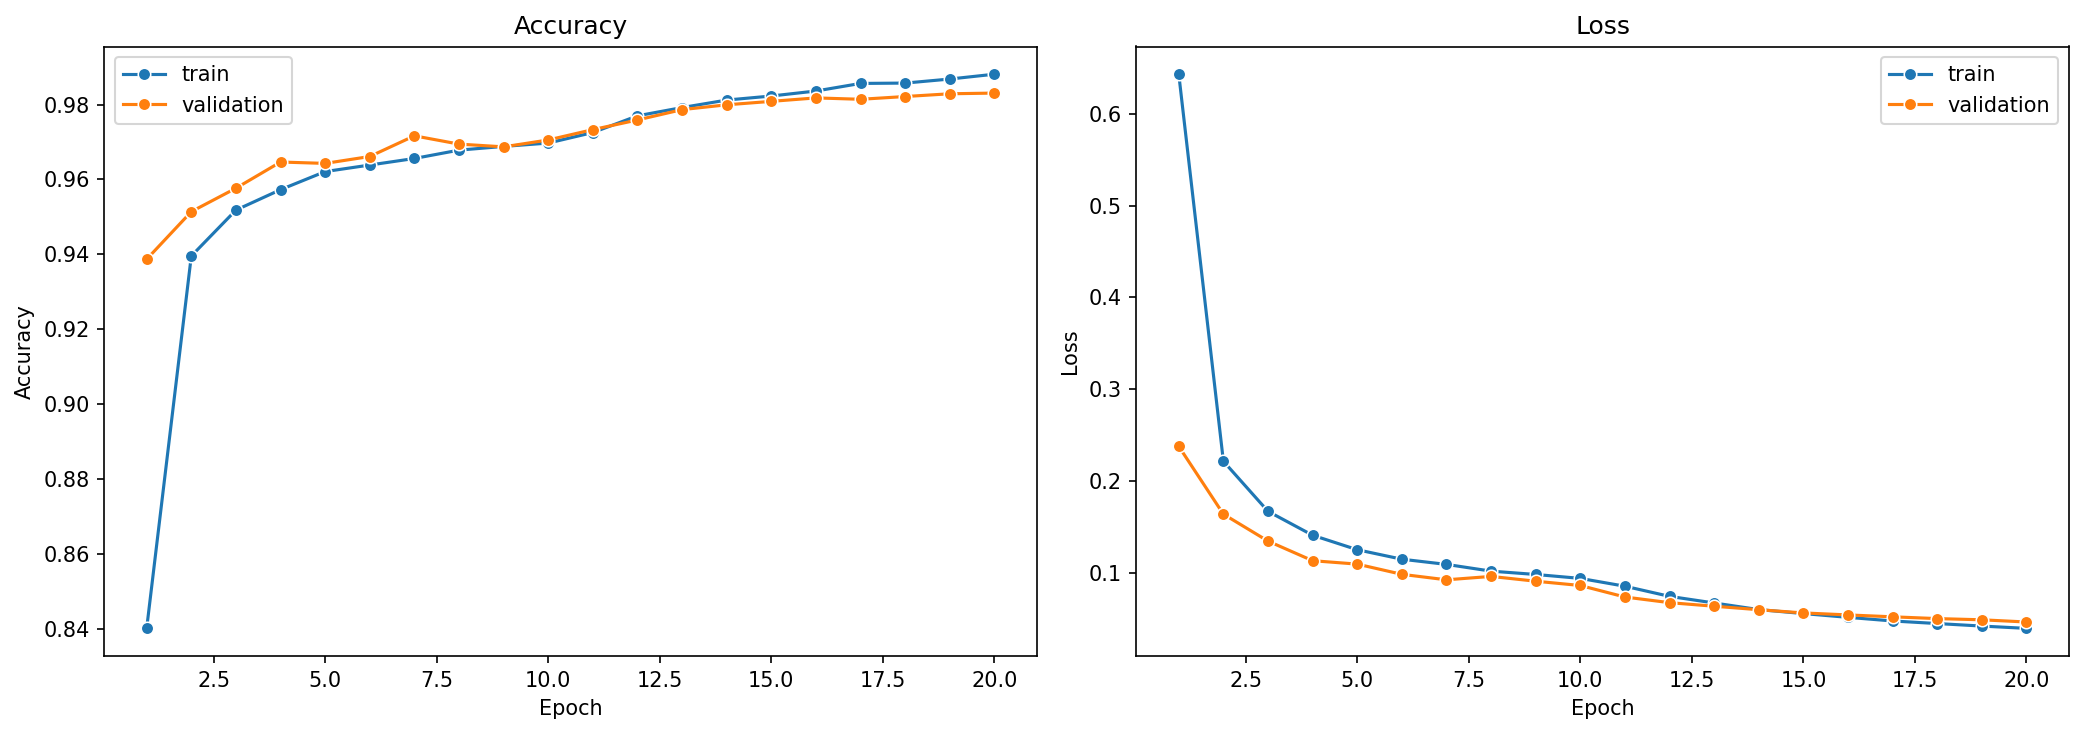
\includegraphics[width=1\textwidth]{../MobileNet/training graph.png}
    \caption{Curvas de exactitud y pérdida durante el entrenamiento de MobileNetV3 Small.\label{fig:mobilenet_training_graph}}
\end{figure}

\subsubsection{Evaluación en el conjunto de prueba}

Al evaluar el modelo sobre el conjunto de prueba, MobileNetV3 Small alcanzó una exactitud de 0,9856 y una pérdida de 0,0485. Este
resultado muestra que el modelo logró generalizar adecuadamente sobre imágenes que no fueron utilizadas durante el entrenamiento. Al
relacionar este valor con las curvas de exactitud y pérdida, se observa que el comportamiento del modelo fue consistente entre
entrenamiento, validación y prueba, ya que la pérdida se mantuvo baja y la exactitud de validación alcanzó valores cercanos a los
obtenidos en el conjunto de prueba.

La matriz de confusión obtenida para MobileNetV3 Small se presenta en la figura \ref{fig:mobilenet_confusion_matrix}. En términos
generales, la diagonal principal concentra la mayor parte de las predicciones correctas, lo que coincide con la exactitud global
obtenida. Las confusiones restantes se concentran principalmente en clases visualmente cercanas, especialmente en enfermedades de
tomate y maíz, donde las hojas pueden presentar manchas, cambios de coloración o lesiones con patrones similares.

\begin{figure}[H]
    \centering
    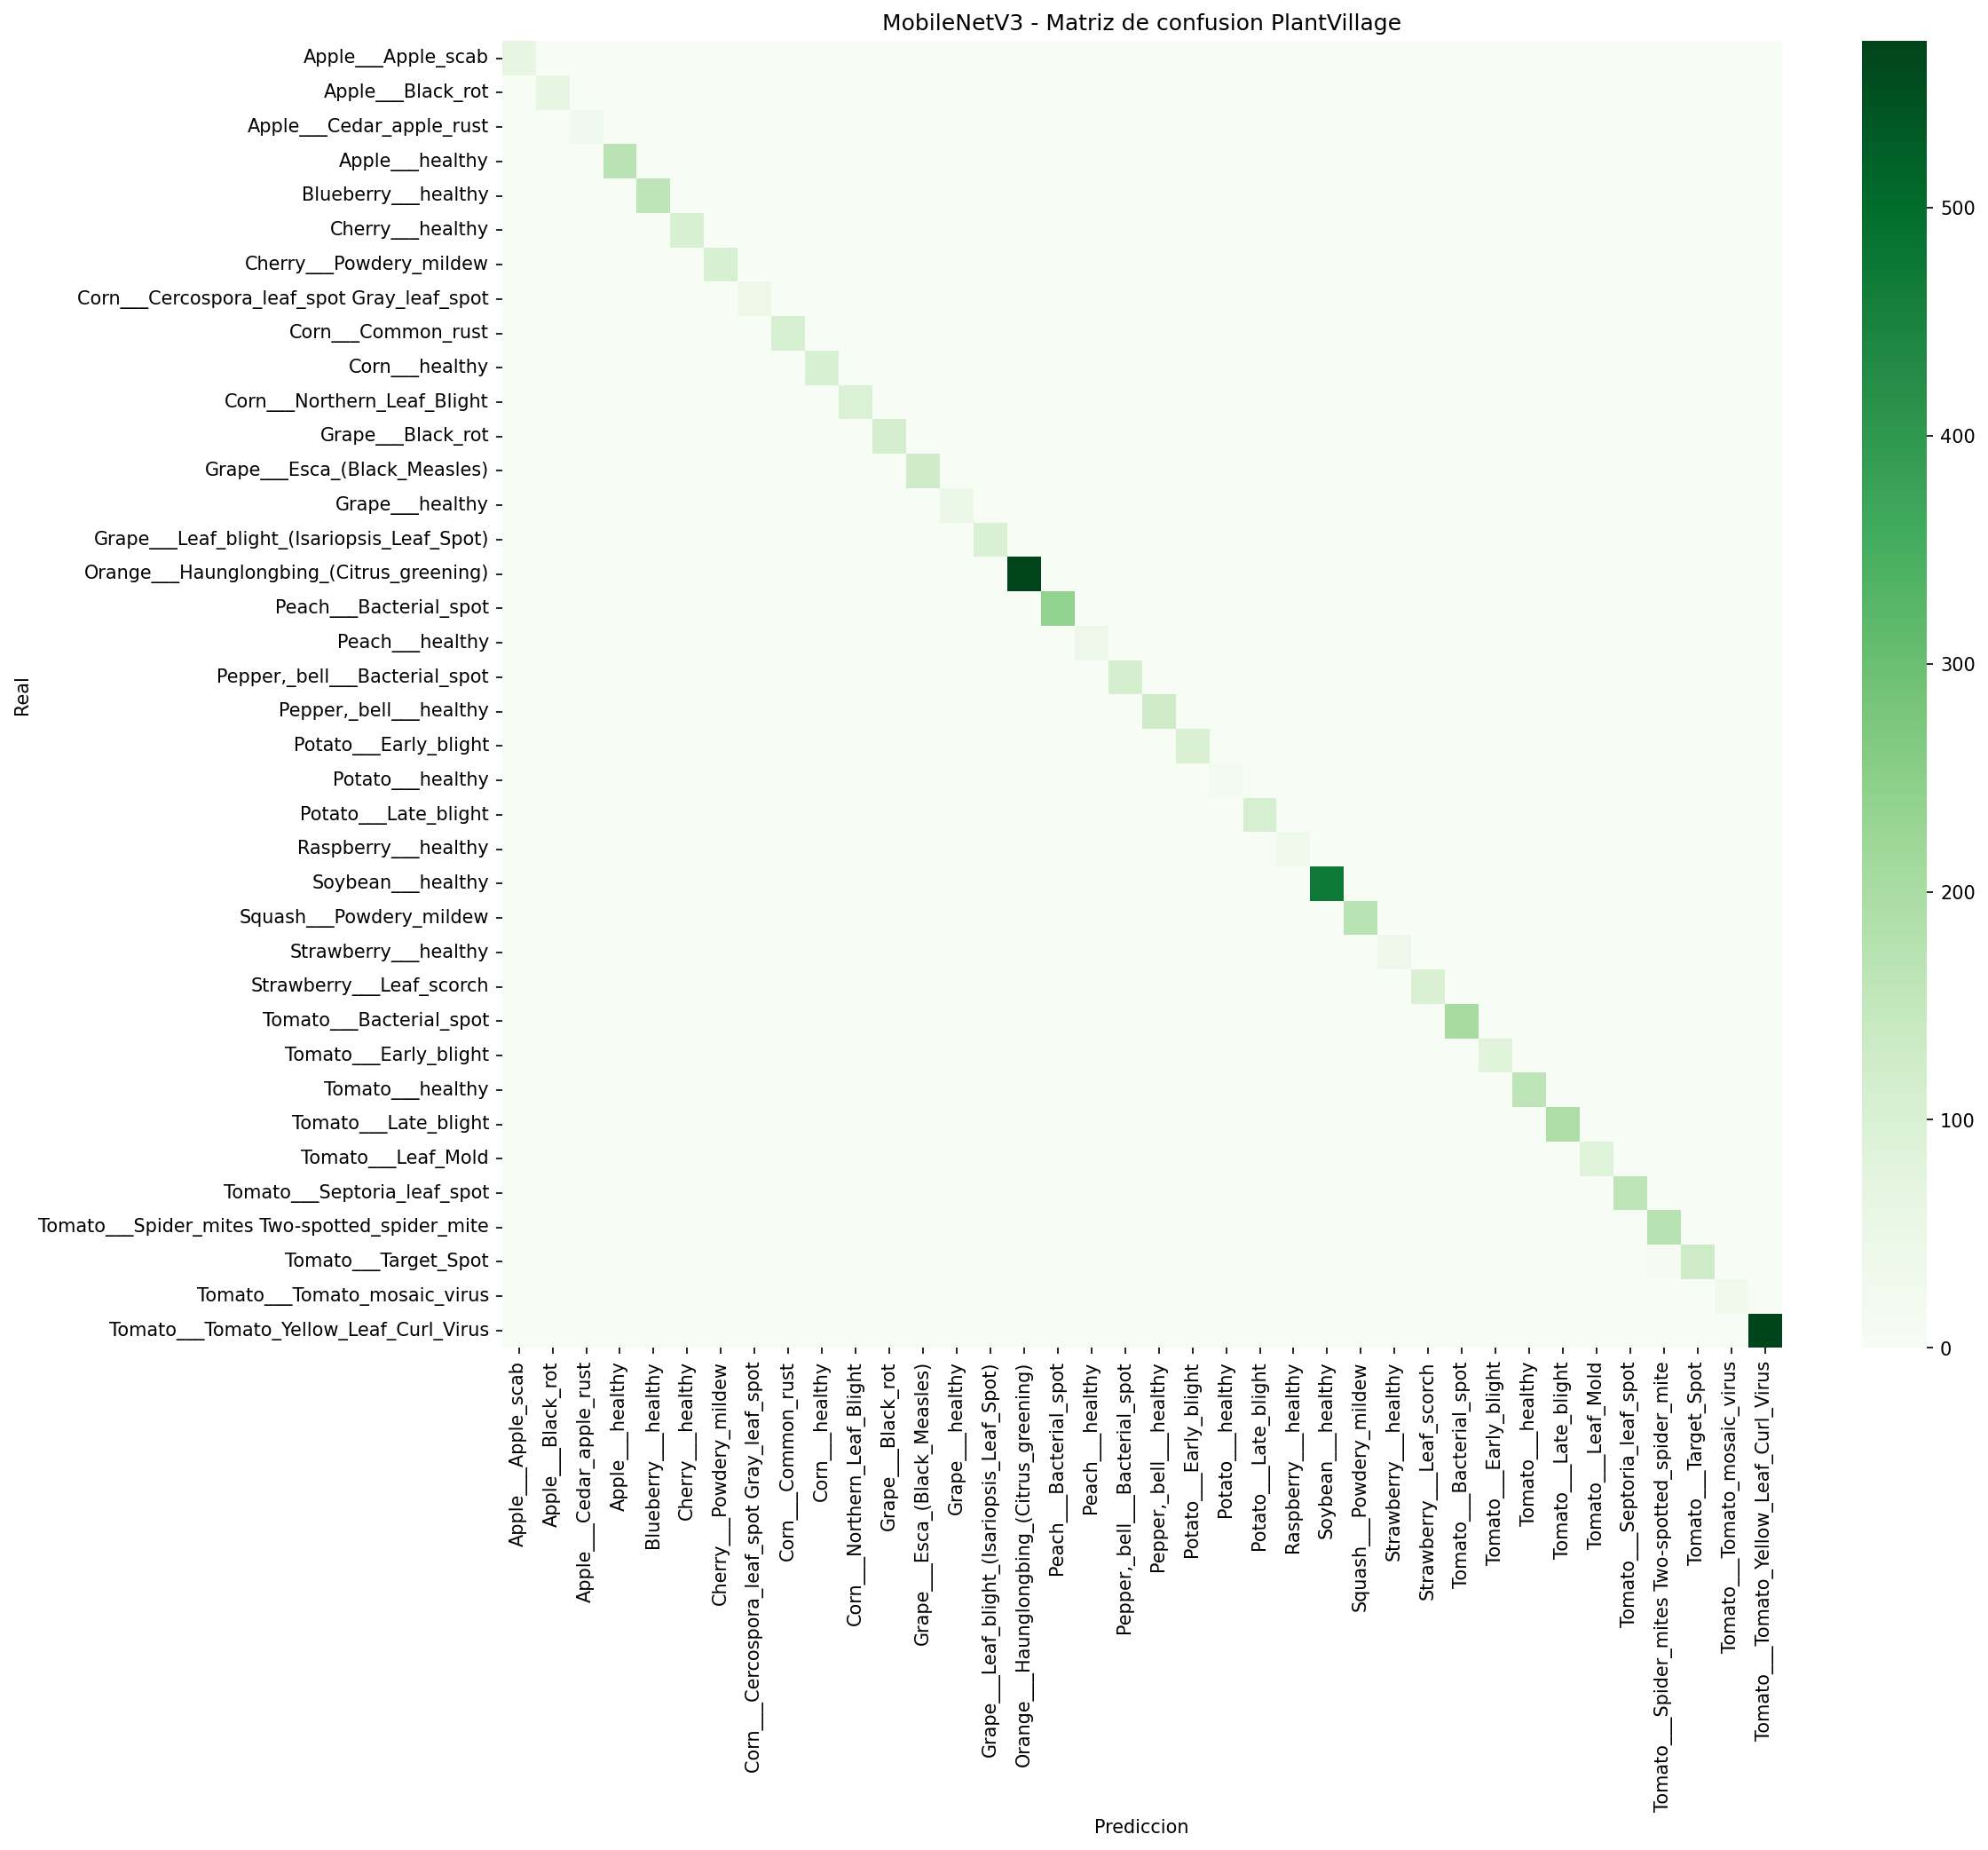
\includegraphics[width=0.95\textwidth]{../MobileNet/confussion_matrix.png}
    \caption{Matriz de confusión del modelo MobileNetV3 Small sobre el conjunto de prueba de PlantVillage.\label{fig:mobilenet_confusion_matrix}}
\end{figure}

\subsubsection{Exportación del modelo}

Después del entrenamiento, el modelo fue exportado a TensorFlow Lite en formato FP32 y FP16. La versión FP16 redujo el tamaño del
archivo de 3,67 MB a 1,91 MB, lo que representa una ventaja importante frente a EfficientNetV2B0 para el despliegue móvil. Esta
diferencia permite que MobileNetV3 Small sea más liviano dentro de la aplicación y mantenga un desempeño de clasificación alto sin
incrementar de forma significativa el tamaño del modelo integrado.

\subsection{Modelo EfficientNetV2B0}

EfficientNetV2B0 fue entrenado como arquitectura de comparación frente a MobileNetV3 Small, manteniendo el mismo conjunto de clases,
la misma división de los datos y el mismo criterio de evaluación descrito en la metodología. Para este modelo se utilizó la variante
B0, con imágenes de entrada de 224x224 píxeles y pesos iniciales preentrenados en ImageNet. A diferencia de MobileNetV3 Small, el
preprocesamiento de EfficientNetV2B0 se realizó normalizando los valores de los píxeles en el rango [0, 1], por lo que esta
diferencia también se conservó durante la integración del modelo en la aplicación móvil.

\subsubsection{Configuración del entrenamiento}

La tabla \ref{tab:efficientnet_training_results} resume los principales resultados del entrenamiento y exportación del modelo
EfficientNetV2B0, considerando tanto la configuración utilizada como las métricas obtenidas sobre el conjunto de prueba.

\begin{table}[H]
    \centering
    \caption{Resumen de entrenamiento y exportación del modelo EfficientNetV2B0.}
    \label{tab:efficientnet_training_results}
    \begin{tabular}{>{\raggedright\arraybackslash}p{6cm} >{\centering\arraybackslash}p{6cm}}
        \hline
        \textbf{Atributo} & \textbf{Resultado} \\
        \hline
        Arquitectura & EfficientNetV2B0 \\
        Variante & B0 \\
        Tamaño de entrada & 224x224 píxeles \\
        Número de clases & 38 \\
        División del conjunto de datos & 80\% entrenamiento, 10\% validación, 10\% prueba \\
        Imágenes de entrenamiento & 43442 \\
        Imágenes de validación & 5430 \\
        Imágenes de prueba & 5431 \\
        Preprocesamiento & Normalización en el rango [0, 1] \\
        Épocas de entrenamiento de cabeza & 15 \\
        Épocas de ajuste fino & 10 \\
        Capas descongeladas en ajuste fino & Últimas 20 capas del backbone \\
        Mejor exactitud de validación & 0,9851 \\
        Exactitud en prueba & 0,9847 \\
        Pérdida en prueba & 0,0490 \\
        Precisión macro & 0,9823 \\
        Recall macro & 0,9758 \\
        F1-score macro & 0,9784 \\
        Errores en prueba & 83 de 5431 imágenes \\
        Tamaño del modelo TFLite FP32 & 22,52 MB \\
        Tamaño del modelo TFLite FP16 & 11,33 MB \\
        \hline
    \end{tabular}
\end{table}

La arquitectura final tuvo 5.973.110 parámetros, de los cuales
en la primera fase solo se entrenaron 51.238 correspondientes a la cabeza de clasificación.


\subsubsection{Evolución del entrenamiento}

El entrenamiento se organizó en dos fases. En la primera fase se congeló el backbone preentrenado y se entrenó únicamente la cabeza
de clasificación agregada para las 38 clases de PlantVillage. Esta etapa inició con una exactitud de validación de 0,9586 en la
primera época y finalizó con 0,9805 en la época 15. Durante esta fase se observaron pequeñas mesetas en la mejora de la validación,
por lo que el ajuste automático de la tasa de aprendizaje redujo el valor inicial de 1e-3 a 3e-4 y posteriormente a 9e-5. Después de
estas reducciones, el modelo volvió a mejorar, lo que muestra que el mecanismo de reducción de learning rate ayudó a continuar la
convergencia.

Posteriormente, en la fase de ajuste fino, se descongelaron las últimas capas del backbone con una tasa de aprendizaje de 1e-5,
manteniendo congeladas las capas de normalización por lotes para evitar cambios bruscos en las estadísticas aprendidas durante el
preentrenamiento. Esta segunda fase aumentó la exactitud de validación desde 0,9805 hasta 0,9851, obtenida en la época 24. La época
25 presentó una disminución leve en la exactitud de validación, mientras que la exactitud de entrenamiento continuó aumentando, por
lo que el mejor checkpoint correspondió a la época 24.

La figura \ref{fig:efficientnet_training_graph} muestra las curvas de exactitud y pérdida durante las dos fases del entrenamiento.
En la curva de exactitud se observa una mejora rápida durante las primeras épocas, seguida de un crecimiento más gradual. En la curva
de pérdida, tanto el error de entrenamiento como el de validación disminuyen de forma estable, sin una separación marcada entre ambas
curvas. Este comportamiento indica que el modelo logró adaptarse al conjunto PlantVillage sin evidenciar un sobreajuste fuerte durante
la ejecución registrada.

\begin{figure}[H]
    \centering
    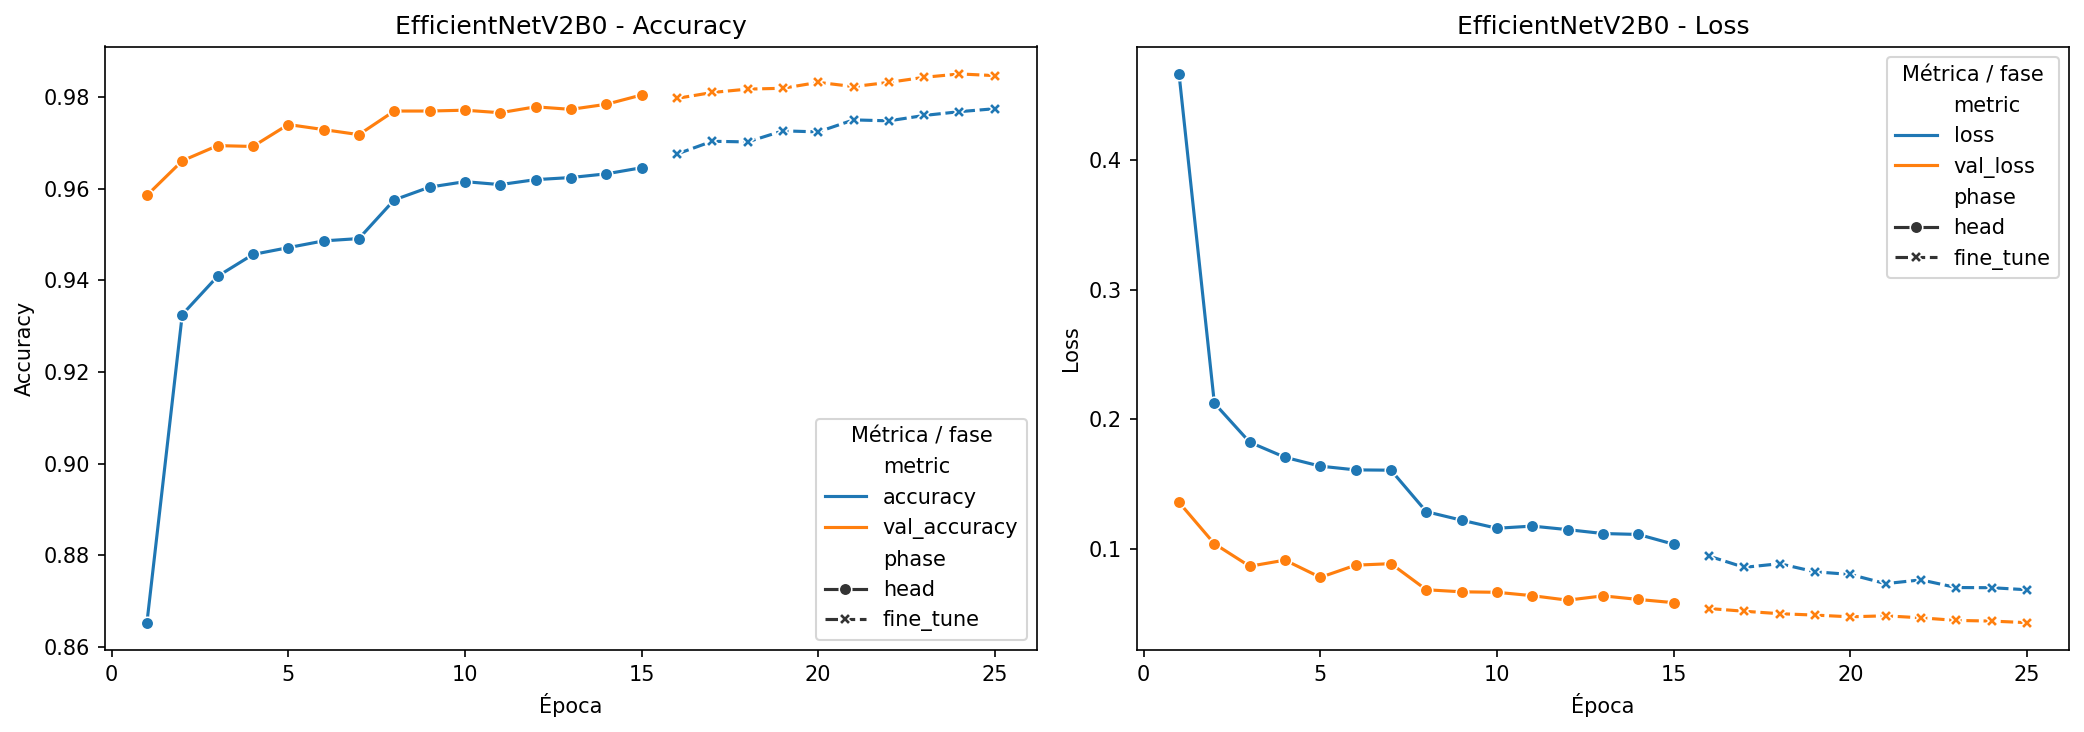
\includegraphics[width=1\textwidth]{../EfficientNet/training_graph_v2b0.png}
    \caption{Curvas de exactitud y pérdida durante el entrenamiento de EfficientNetV2B0.\label{fig:efficientnet_training_graph}}
\end{figure}

\subsubsection{Evaluación en el conjunto de prueba}

Al evaluar el mejor checkpoint sobre el conjunto de prueba, el modelo alcanzó una exactitud de 0,9847 y una pérdida de 0,0490. En
términos generales, este resultado muestra que EfficientNetV2B0 consiguió un desempeño alto sobre PlantVillage, con 83 errores en
5.431 imágenes evaluadas. Además, las métricas agregadas se mantuvieron cercanas entre sí, con una precisión macro de 0,9823, recall
macro de 0,9758 y F1-score macro de 0,9784.

Aunque el resultado global fue alto, el análisis por clase muestra que los errores no se distribuyeron de manera uniforme. La tabla
\ref{tab:efficientnet_weak_classes} presenta las clases con F1-score menor a 0,96, que corresponden a los casos donde el modelo tuvo
mayor dificultad relativa.

\begin{table}[H]
    \centering
    \caption{Clases con menor desempeño relativo en EfficientNetV2B0.}
    \label{tab:efficientnet_weak_classes}
    \begin{tabular}{>{\raggedright\arraybackslash}p{5.7cm}
                    >{\centering\arraybackslash}p{1.6cm}
                    >{\centering\arraybackslash}p{1.6cm}
                    >{\centering\arraybackslash}p{1.6cm}
                    >{\centering\arraybackslash}p{1.6cm}}
        \hline
        \textbf{Clase} & \textbf{Prec.} & \textbf{Recall} & \textbf{F1} & \textbf{Soporte} \\
        \hline
        Potato healthy & 1,0000 & 0,7273 & 0,8421 & 11 \\
        Tomato Target Spot & 0,8855 & 0,8855 & 0,8855 & 131 \\
        Corn Cercospora leaf spot Gray leaf spot & 0,9375 & 0,9000 & 0,9184 & 50 \\
        Tomato Early blight & 0,9691 & 0,8952 & 0,9307 & 105 \\
        Tomato Septoria leaf spot & 0,9459 & 0,9396 & 0,9428 & 149 \\
        Tomato Leaf Mold & 0,9341 & 0,9551 & 0,9444 & 89 \\
        Tomato Spider mites Two-spotted spider mite & 0,9382 & 0,9543 & 0,9462 & 175 \\
        \hline
    \end{tabular}
\end{table}

En la tabla, Prec. corresponde a precisión.

El caso de Potato healthy (Papa sana) fue el de menor F1-score; sin embargo, esta clase tuvo solo 11 ejemplos en el conjunto de prueba, por lo
que cada error individual tuvo un impacto alto sobre el recall. En cambio, Tomato Target Spot representa un caso más relevante para
el análisis, debido a que tuvo un soporte mayor y presentó confusiones con otras enfermedades de tomate. Este patrón también se
observó en Tomato Septoria leaf spot, Tomato Leaf Mold y Tomato Spider mites, donde las lesiones foliares pueden tener una apariencia
visual similar. En maíz, la confusión principal apareció entre Corn Cercospora leaf spot Gray leaf spot y Corn Northern Leaf Blight,
lo cual es consistente con la similitud visual entre lesiones alargadas y manchas grises en las hojas.

La matriz de confusión obtenida para EfficientNetV2B0 se presenta en la figura \ref{fig:efficientnet_confusion_matrix}. Esta matriz
permite identificar visualmente las clases en las que el modelo concentró la mayor parte de sus aciertos y los casos en los que se
presentaron confusiones entre enfermedades o cultivos con características visuales similares. Este análisis es relevante porque una
exactitud global alta no siempre evidencia los errores específicos que pueden aparecer en clases particulares.

\begin{figure}[H]
    \centering
    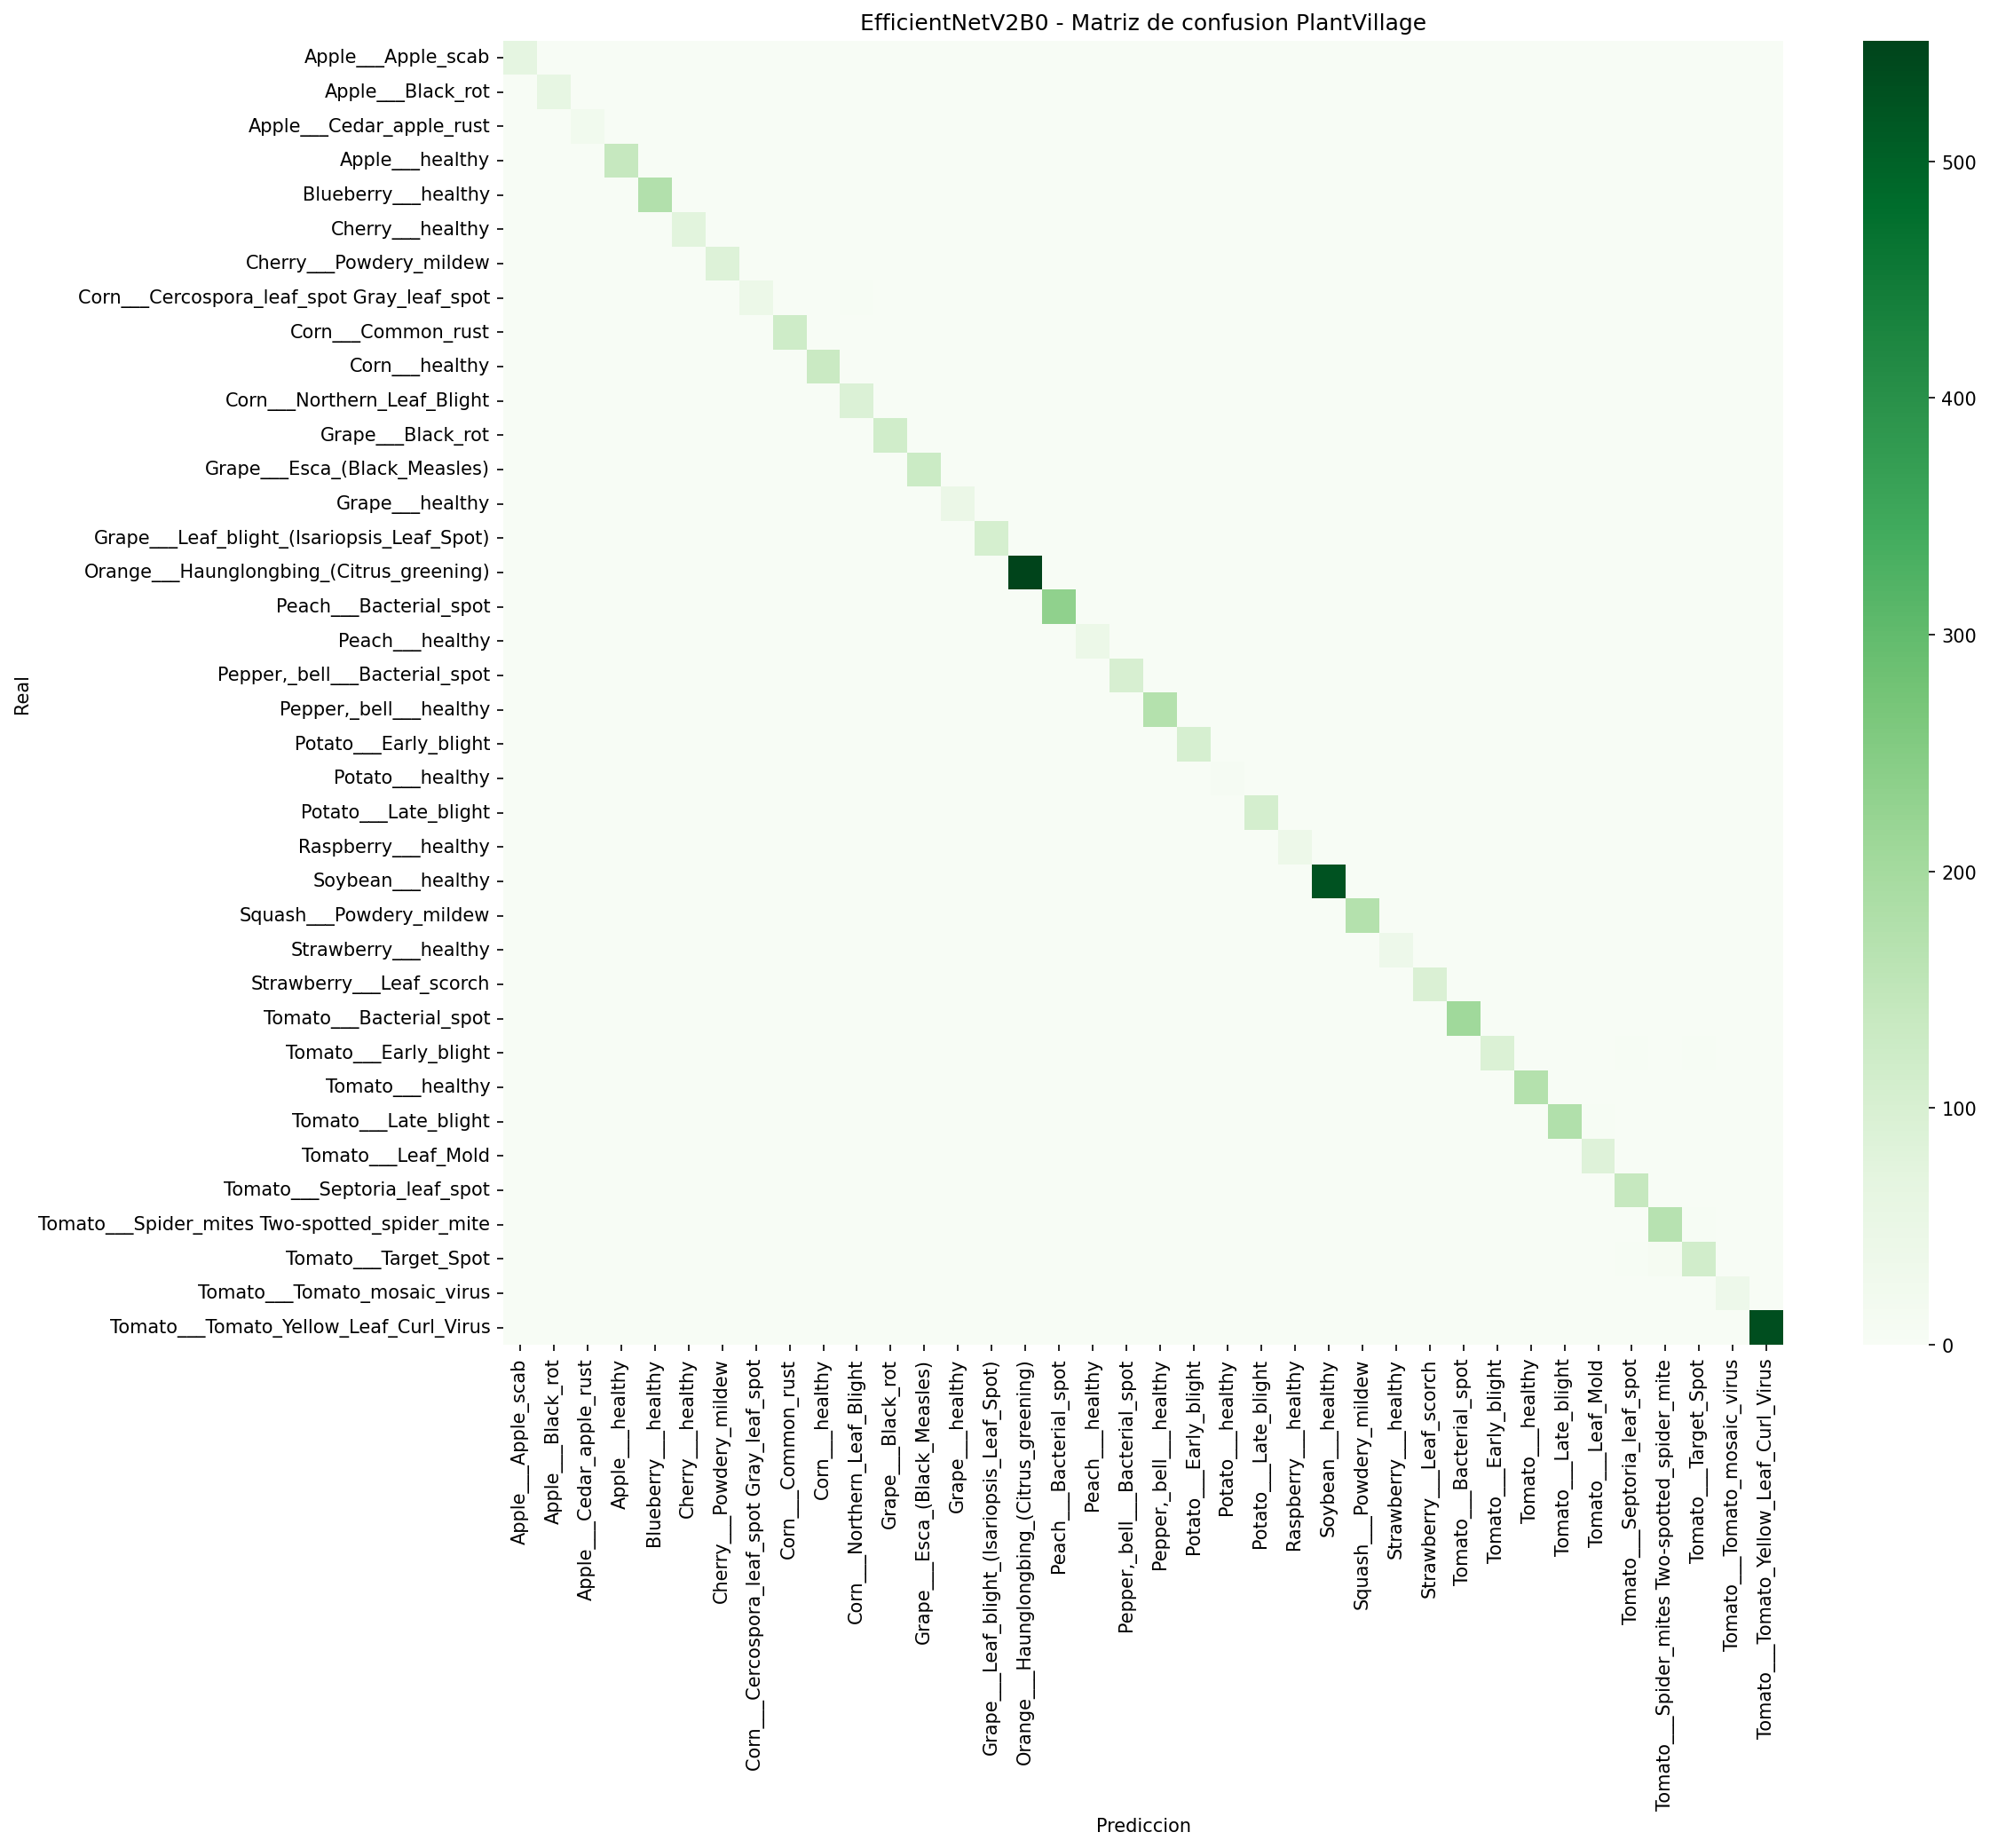
\includegraphics[width=0.95\textwidth]{../EfficientNet/confusion_matrix_v2b0.png}
    \caption{Matriz de confusión del modelo EfficientNetV2B0 sobre el conjunto de prueba de PlantVillage.\label{fig:efficientnet_confusion_matrix}}
\end{figure}

\subsubsection{Exportación del modelo}

Después del entrenamiento, el modelo fue exportado a TensorFlow Lite en formato FP32 y FP16. La versión FP16 redujo el tamaño del
archivo aproximadamente a la mitad, pasando de 22,52 MB a 11,33 MB. Esta reducción es importante para el despliegue en dispositivos
móviles, ya que disminuye el espacio requerido por el modelo dentro de la aplicación y facilita su distribución sin modificar la
estructura general de la arquitectura entrenada. Sin embargo, este modelo requiere conservar el preprocesamiento en el rango [0, 1],
por lo que su uso en Android depende de aplicar una normalización diferente a la utilizada por MobileNetV3 Small.

\section{Aplicación móvil}
En la figura \ref{fig:app_screenshots} se muestran capturas de pantalla de la aplicación móvil desarrollada para la ejecución de
inferencias en los dispositivos. La pantalla inicial (captura a) permite seleccionar el modelo que se desea probar, ya sea
MobileNetV3 Small o EfficientNetV2B0. Desde esta misma vista, el usuario puede ingresar la imagen al modelo mediante dos opciones:
cargar una fotografía desde la galería del dispositivo (captura b) o capturar una imagen directamente desde la cámara de la
aplicación (captura c). En la pantalla de captura se mantiene un área de enfoque que orienta al usuario para ubicar la hoja dentro
de la región de análisis, con el fin de facilitar una entrada más adecuada para el proceso de inferencia.

\begin{figure}[H]
    \centering
    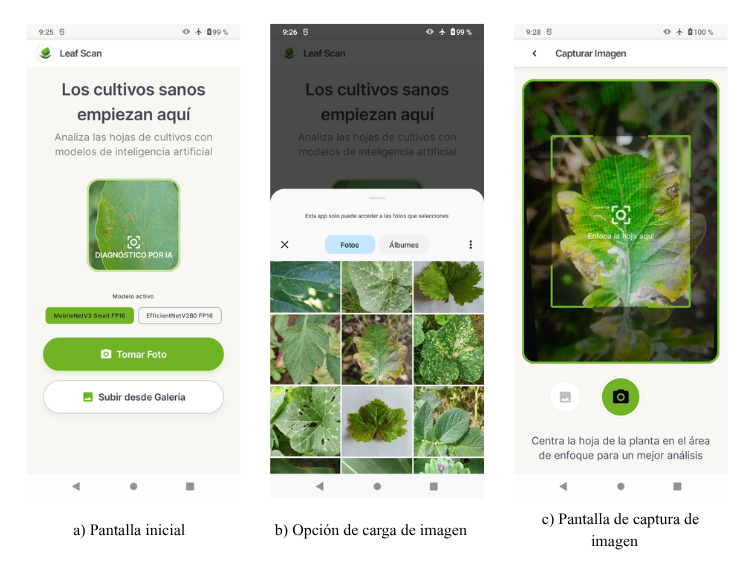
\includegraphics[width=1\textwidth]{images/app_screenshots.png}
    \caption{Pantallas iniciales de la aplicación móvil: selección del modelo, carga desde galería y captura de imagen.\label{fig:app_screenshots}}
\end{figure}


Posteriormente, en la figura \ref{fig:app_screenshots_2} se presenta el flujo de análisis de la imagen. La pantalla de análisis
(captura a) muestra la imagen seleccionada y el avance de la ejecución del modelo, de manera que el usuario pueda identificar que la
inferencia se encuentra en proceso. Cuando la predicción obtiene una confianza igual o superior al umbral definido del 50\%, se
presenta la pantalla de resultado (captura b), en la cual se indica la clase asignada, el porcentaje de confianza asociado y una
descripción breve relacionada con el diagnóstico obtenido.

En caso de que la confianza de la predicción sea menor al 50\%, o si durante la ejecución del modelo se presenta un error, la
aplicación muestra un mensaje de error en la pantalla de análisis (captura c). Aquí se informa que no fue posible clasificar la 
imagen y se habilita la
opción de reintento, permitiendo al usuario tomar o seleccionar una nueva fotografía. De esta forma, la interfaz mantiene un flujo
simple para la prueba de los modelos, desde la selección de la imagen hasta la visualización del diagnóstico o la repetición del
proceso cuando la entrada no permite una inferencia confiable.

\begin{figure}[H]
    \centering
    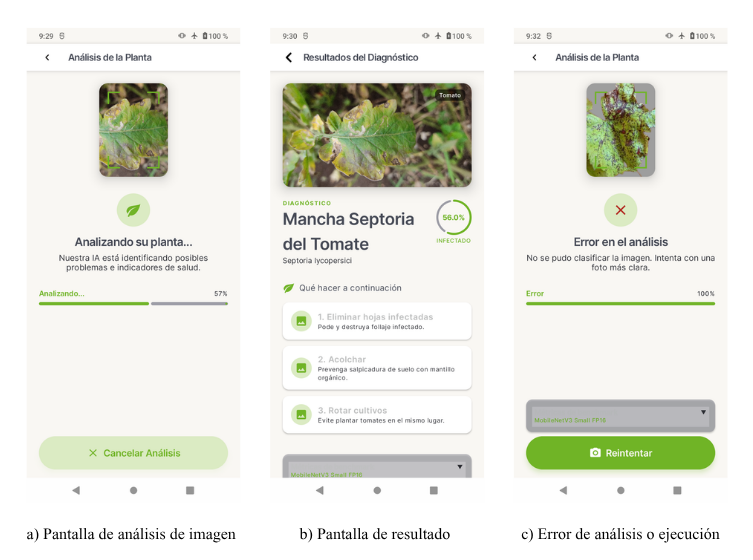
\includegraphics[width=1\textwidth]{images/app_screenshots_2.png}
    \caption{Pantallas de análisis, resultado y error durante la inferencia en la aplicación móvil.\label{fig:app_screenshots_2}}
\end{figure}

\section{Resultados de ejecución en dispositivo}

    La tabla \ref{tab:motog_execution_results} presenta las mediciones obtenidas en el dispositivo Moto G30 durante tres sesiones de
    evaluación. En cada sesión se ejecutaron ambos modelos bajo el mismo protocolo de prueba, registrando variables asociadas al estado del
dispositivo y al tiempo de inferencia. Durante la ejecucion del protocolo de prueba, se mantuvo el dispositivo en un entorno controlado, 
evitando la ejecución de otras aplicaciones que pudieran afectar el rendimiento. Durante la 
ejecucion de las tres sesiones se mantuvo el mismo nivel de brillo establecido en 60\% y se deshabilitaron las conexiones inalámbricas para evitar interferencias externas,
tambien se desctivo el modo Rendimiento permitiendo el uso de todos los núcleos del procesador.
En ninguna de las sesiones se registraron crashes de la aplicación, ni por errores de codigo ni por falta de recursos.
En las tablas, MNetV3 corresponde a MobileNetV3 Small y EffNet corresponde a EfficientNetV2B0.

\begin{table}[H]
    \centering
    \caption{Resultados de ejecución de MobileNetV3 Small y EfficientNetV2B0 en Moto G30.}
    \label{tab:motog_execution_results}
    \scriptsize
    \resizebox{\textwidth}{!}{%
    \begin{tabular}{>{\raggedright\arraybackslash}p{3.2cm}
                    >{\centering\arraybackslash}p{1.8cm}
                    >{\centering\arraybackslash}p{1.8cm}
                    >{\centering\arraybackslash}p{1.8cm}
                    >{\centering\arraybackslash}p{1.8cm}
                    >{\centering\arraybackslash}p{1.8cm}
                    >{\centering\arraybackslash}p{1.8cm}}
        \hline
        \multicolumn{7}{c}{\textbf{Moto G30}} \\
        \hline
        \textbf{Métrica} & \multicolumn{2}{c}{\textbf{Sesión 1}} & \multicolumn{2}{c}{\textbf{Sesión 2}} & \multicolumn{2}{c}{\textbf{Sesión 3}} \\
        \hline
        & \textbf{MNetV3} & \textbf{EffNet} & \textbf{MNetV3} & \textbf{EffNet} & \textbf{MNetV3} & \textbf{EffNet} \\
        \hline
        Temperatura inicial (C) & 283 & 284 & 272 & 290 & 258 & 300 \\
        Temperatura final (C) & 296 & 316 & 295 & 324 & 295 & 313 \\
        Batería inicial (\%) & 100 & 79 & 72 & 65 & 50 & 65 \\
        Batería final (\%) & 77 & 68 & 63 & 55 & 37 & 51 \\
        Tiempo de inicialización (ms) & 3423 & 357 & 3220 & 319 & 3258 & 374 \\
        Warmup (ms) & 258,8 & 495,8 & 248 & 463,1 & 60,4 & 671,4 \\
        Latencia promedio (ms) & 24,8 & 273,6 & 31,9 & 276,8 & 35,3 & 272 \\
        Mediana P50 (ms) & 23,2 & 266,6 & 31 & 271,8 & 31,8 & 265,2 \\
        Percentil P95 (ms) & 36,9 & 311,4 & 52,5 & 323,9 & 69 & 318,1 \\
        Desviación estándar (ms) & 7,5 & 22,6 & 12,3 & 22,8 & 18,1 & 23,2 \\
        \hline
    \end{tabular}%
    }
\end{table}

La tabla \ref{tab:motog_cross_session_results} resume el promedio entre sesiones para las métricas principales de latencia en el
Moto G30. Aquí se observa de forma más directa la diferencia global entre ambos modelos, donde MobileNetV3 Small mantiene latencias promedio 
considerablemente menores, mientras que EfficientNetV2B0 presenta tiempos más altos y una variabilidad mayor. En términos de latencia promedio,
MobileNetV3 Small fue aproximadamente 8,94 veces más rápido que EfficientNetV2B0, lo que evidencia una brecha significativa en el rendimiento
de inferencia entre ambos modelos en este dispositivo móvil. Esta diferencia se mantiene también en la mediana P50 y el percentil P95, 
aunque con una variabilidad mayor en el caso de EfficientNetV2B0, lo que sugiere que este modelo no solo es más lento en promedio, sino que también
presenta una mayor inconsistencia en sus tiempos de inferencia.
\begin{table}[H]
    \centering
    \caption{Promedio entre sesiones de las métricas de ejecución en Moto G30.}
    \label{tab:motog_cross_session_results}
    \resizebox{\textwidth}{!}{%
    \begin{tabular}{>{\raggedright\arraybackslash}p{4cm}
                    >{\centering\arraybackslash}p{3cm}
                    >{\centering\arraybackslash}p{3cm}
                    >{\centering\arraybackslash}p{3cm}}
        \hline
        \textbf{Métrica} & \textbf{MNetV3} & \textbf{EffNet} & \textbf{Ratio Eff/MNV3} \\
        \hline
        Latencia promedio (ms) & 30,67 & 274,13 & 8,94x \\
        Mediana P50 (ms) & 28,67 & 267,87 & 9,34x \\
        Percentil P95 (ms) & 52,80 & 317,80 & 6,02x \\
        Desviación estándar (ms) & 12,63 & 22,87 & -- \\
        \hline
    \end{tabular}%
    }
\end{table}

La tabla \ref{tab:samsung_execution_results} presenta las mediciones obtenidas en el dispositivo Samsung Galaxy S23 durante las tres
sesiones de evaluación. 

\begin{table}[H]
    \centering
    \caption{Resultados de ejecución de MobileNetV3 Small y EfficientNetV2B0 en Samsung Galaxy S23.}
    \label{tab:samsung_execution_results}
    \scriptsize
    \resizebox{\textwidth}{!}{%
    \begin{tabular}{>{\raggedright\arraybackslash}p{3.2cm}
                    >{\centering\arraybackslash}p{1.8cm}
                    >{\centering\arraybackslash}p{1.8cm}
                    >{\centering\arraybackslash}p{1.8cm}
                    >{\centering\arraybackslash}p{1.8cm}
                    >{\centering\arraybackslash}p{1.8cm}
                    >{\centering\arraybackslash}p{1.8cm}}
        \hline
        \multicolumn{7}{c}{\textbf{Samsung Galaxy S23}} \\
        \hline
        \textbf{Métrica} & \multicolumn{2}{c}{\textbf{Sesión 1}} & \multicolumn{2}{c}{\textbf{Sesión 2}} & \multicolumn{2}{c}{\textbf{Sesión 3}} \\
        \hline
        & \textbf{MNetV3} & \textbf{EffNet} & \textbf{MNetV3} & \textbf{EffNet} & \textbf{MNetV3} & \textbf{EffNet} \\
        \hline
        Temperatura inicial (C) & 289 & 247 & 250 & 292 & 262 & 293 \\
        Temperatura final (C) & 300 & 335 & 313 & 313 & 313 & 310 \\
        Batería inicial (\%) & 100 & 93 & 90 & 83 & 75 & 82 \\
        Batería final (\%) & 93 & 85 & 83 & 75 & 68 & 75 \\
        Tiempo de inicialización (ms) & 844 & 140 & 863 & 141 & 647 & 172 \\
        Warmup (ms) & 45,4 & 92,5 & 44,9 & 87,6 & 10 & 145,7 \\
        Latencia promedio (ms) & 7,8 & 52,5 & 7,9 & 52,4 & 7,8 & 53,5 \\
        Mediana P50 (ms) & 6,6 & 48,6 & 6,6 & 48,7 & 6,5 & 49,4 \\
        Percentil P95 (ms) & 14,2 & 68,7 & 14,2 & 68,9 & 13,5 & 69 \\
        Desviación estándar (ms) & 3,6 & 9,3 & 3,4 & 9 & 3,1 & 8,6 \\
        \hline
    \end{tabular}%
    }
\end{table}

La tabla \ref{tab:samsung_cross_session_results} resume el promedio entre sesiones para las métricas principales de latencia en el
Samsung Galaxy S23.

\begin{table}[H]
    \centering
    \caption{Promedio entre sesiones de las métricas de ejecución en Samsung Galaxy S23.}
    \label{tab:samsung_cross_session_results}
    \resizebox{\textwidth}{!}{%
    \begin{tabular}{>{\raggedright\arraybackslash}p{4cm}
                    >{\centering\arraybackslash}p{3cm}
                    >{\centering\arraybackslash}p{3cm}
                    >{\centering\arraybackslash}p{3cm}}
        \hline
        \textbf{Métrica} & \textbf{MNetV3} & \textbf{EffNet} & \textbf{Ratio Eff/MNV3} \\
        \hline
        Latencia promedio (ms) & 7,83 & 52,80 & 6,74x \\
        Mediana P50 (ms) & 6,57 & 48,90 & 7,44x \\
        Percentil P95 (ms) & 13,97 & 68,87 & 4,93x \\
        Desviación estándar (ms) & 3,37 & 8,97 & -- \\
        \hline
    \end{tabular}%
    }
\end{table}

Al comparar los resultados de la tabla \ref{tab:samsung_cross_session_results} con los obtenidos en el Moto G30 en la tabla
\ref{tab:motog_cross_session_results}, se evidencia una reducción considerable en los tiempos de inferencia en el dispositivo con
mejor procesador. En MobileNetV3 Small, la latencia registrada en el Moto G30 equivale aproximadamente a 32 clasificaciones por
segundo, por lo que permite un flujo de uso casi continuo en campo. En el Samsung Galaxy S23, esta misma arquitectura alcanza cerca
de 127 clasificaciones por segundo, lo que hace que la inferencia sea prácticamente instantánea desde la perspectiva del usuario.

En EfficientNetV2B0, el comportamiento también mejora de forma importante, aunque sus tiempos siguen siendo mayores que los de
MobileNetV3 Small. En el Moto G30, el modelo alcanza alrededor de 3,6 clasificaciones por segundo, por lo que su uso se ajusta mejor
a una captura estática con una espera perceptible. En el Samsung Galaxy S23, en cambio, alcanza cerca de 19 clasificaciones por
segundo, lo que resulta fluido para un uso en campo. La brecha entre modelos es mayor en el dispositivo de gama media que en el
dispositivo de gama alta; sin embargo, el mejor hardware reduce la diferencia relativa sin eliminarla. Además, la mejora entre
dispositivos fue mayor para EfficientNetV2B0 que para MobileNetV3 Small, lo que sugiere que el modelo de mayor tamaño aprovecha en
mayor medida las capacidades del SoC más avanzado.

\subsection{Tiempo de inicialización y warmup}

Además de la latencia promedio de inferencia, se registraron dos tiempos adicionales durante la ejecución de los modelos: el tiempo de
inicialización y el warmup. El tiempo de inicialización corresponde a la carga del modelo en memoria, la cual ocurre una sola vez al
iniciar la aplicación o al seleccionar el modelo. Por su parte, el warmup corresponde a la primera inferencia ejecutada, que puede ser
más lenta que las siguientes debido a la preparación inicial del intérprete, la compilación y el precalentamiento de cachés.

La tabla \ref{tab:motog_init_warmup} presenta los tiempos de inicialización y warmup registrados en el Moto G30 para cada sesión de
prueba.

\begin{table}[H]
    \centering
    \caption{Tiempo de inicialización y warmup en Moto G30.}
    \label{tab:motog_init_warmup}
    \scriptsize
    \resizebox{\textwidth}{!}{%
    \begin{tabular}{>{\raggedright\arraybackslash}p{3cm}
                    >{\centering\arraybackslash}p{1.8cm}
                    >{\centering\arraybackslash}p{1.8cm}
                    >{\centering\arraybackslash}p{1.8cm}
                    >{\centering\arraybackslash}p{1.8cm}
                    >{\centering\arraybackslash}p{1.8cm}
                    >{\centering\arraybackslash}p{1.8cm}
                    >{\centering\arraybackslash}p{1.6cm}
                    >{\centering\arraybackslash}p{1.6cm}}
        \hline
        \textbf{Métrica} & \textbf{Sesión 1 MNV3} & \textbf{Sesión 1 Eff} & \textbf{Sesión 2 MNV3} & \textbf{Sesión 2 Eff} & \textbf{Sesión 3 MNV3} & \textbf{Sesión 3 Eff} & \textbf{Avg MNV3} & \textbf{Avg Eff} \\
        \hline
        Tiempo de inicialización (ms) & 3423 & 357 & 3220 & 319 & 3258 & 374 & 3300 & 350 \\
        Warmup (ms) & 258,8 & 495,8 & 248,0 & 463,1 & 60,4 & 671,4 & 189 & 543 \\
        \hline
    \end{tabular}%
    }
\end{table}

La tabla \ref{tab:samsung_init_warmup} presenta las mismas métricas registradas en el Samsung Galaxy S23.

\begin{table}[H]
    \centering
    \caption{Tiempo de inicialización y warmup en Samsung Galaxy S23.}
    \label{tab:samsung_init_warmup}
    \scriptsize
    \resizebox{\textwidth}{!}{%
    \begin{tabular}{>{\raggedright\arraybackslash}p{3cm}
                    >{\centering\arraybackslash}p{1.8cm}
                    >{\centering\arraybackslash}p{1.8cm}
                    >{\centering\arraybackslash}p{1.8cm}
                    >{\centering\arraybackslash}p{1.8cm}
                    >{\centering\arraybackslash}p{1.8cm}
                    >{\centering\arraybackslash}p{1.8cm}
                    >{\centering\arraybackslash}p{1.6cm}
                    >{\centering\arraybackslash}p{1.6cm}}
        \hline
        \textbf{Métrica} & \textbf{Sesión 1 MNV3} & \textbf{Sesión 1 Eff} & \textbf{Sesión 2 MNV3} & \textbf{Sesión 2 Eff} & \textbf{Sesión 3 MNV3} & \textbf{Sesión 3 Eff} & \textbf{Avg MNV3} & \textbf{Avg Eff} \\
        \hline
        Tiempo de inicialización (ms) & 844 & 140 & 863 & 141 & 647 & 172 & 785 & 151 \\
        Warmup (ms) & 45,4 & 92,5 & 44,9 & 87,6 & 10,0 & 145,7 & 34 & 109 \\
        \hline
    \end{tabular}%
    }
\end{table}

Los resultados muestran que MobileNetV3 Small presentó un tiempo de inicialización mayor que EfficientNetV2B0 en ambos dispositivos.
En el Moto G30, esta diferencia fue más marcada, ya que MobileNetV3 Small registró un promedio de inicialización de 3300 ms frente a
350 ms de EfficientNetV2B0. Esta diferencia se explica por el uso de \texttt{CompiledModel}, que requiere preparar y enlazar los
kernels antes de ejecutar el modelo, mientras que EfficientNetV2B0 se ejecutó mediante \texttt{Interpreter}, cargando el grafo de
forma más directa. En el Samsung Galaxy S23, los tiempos de inicialización disminuyeron para ambos modelos, especialmente en
MobileNetV3 Small, lo que evidencia que el hardware de mayor capacidad reduce de forma más pronunciada el costo inicial de
compilación. Sin embargo, este tiempo corresponde a un costo único por sesión de uso y no afecta directamente la experiencia durante
la clasificación continua de imágenes, ya que el usuario abre la aplicación una vez y luego puede realizar múltiples inferencias.


\subsection{Memoria PSS}

La figura \ref{fig:pss_motog_models} presenta la distribución de memoria PSS registrada en el Moto G30 para MobileNetV3 Small y
EfficientNetV2B0 durante las tres sesiones de evaluación. Esta métrica permite observar el consumo proporcional de memoria del
proceso de la aplicación durante la ejecución de cada modelo.

\begin{figure}[H]
    \centering
    \begin{minipage}{0.49\textwidth}
        \centering
        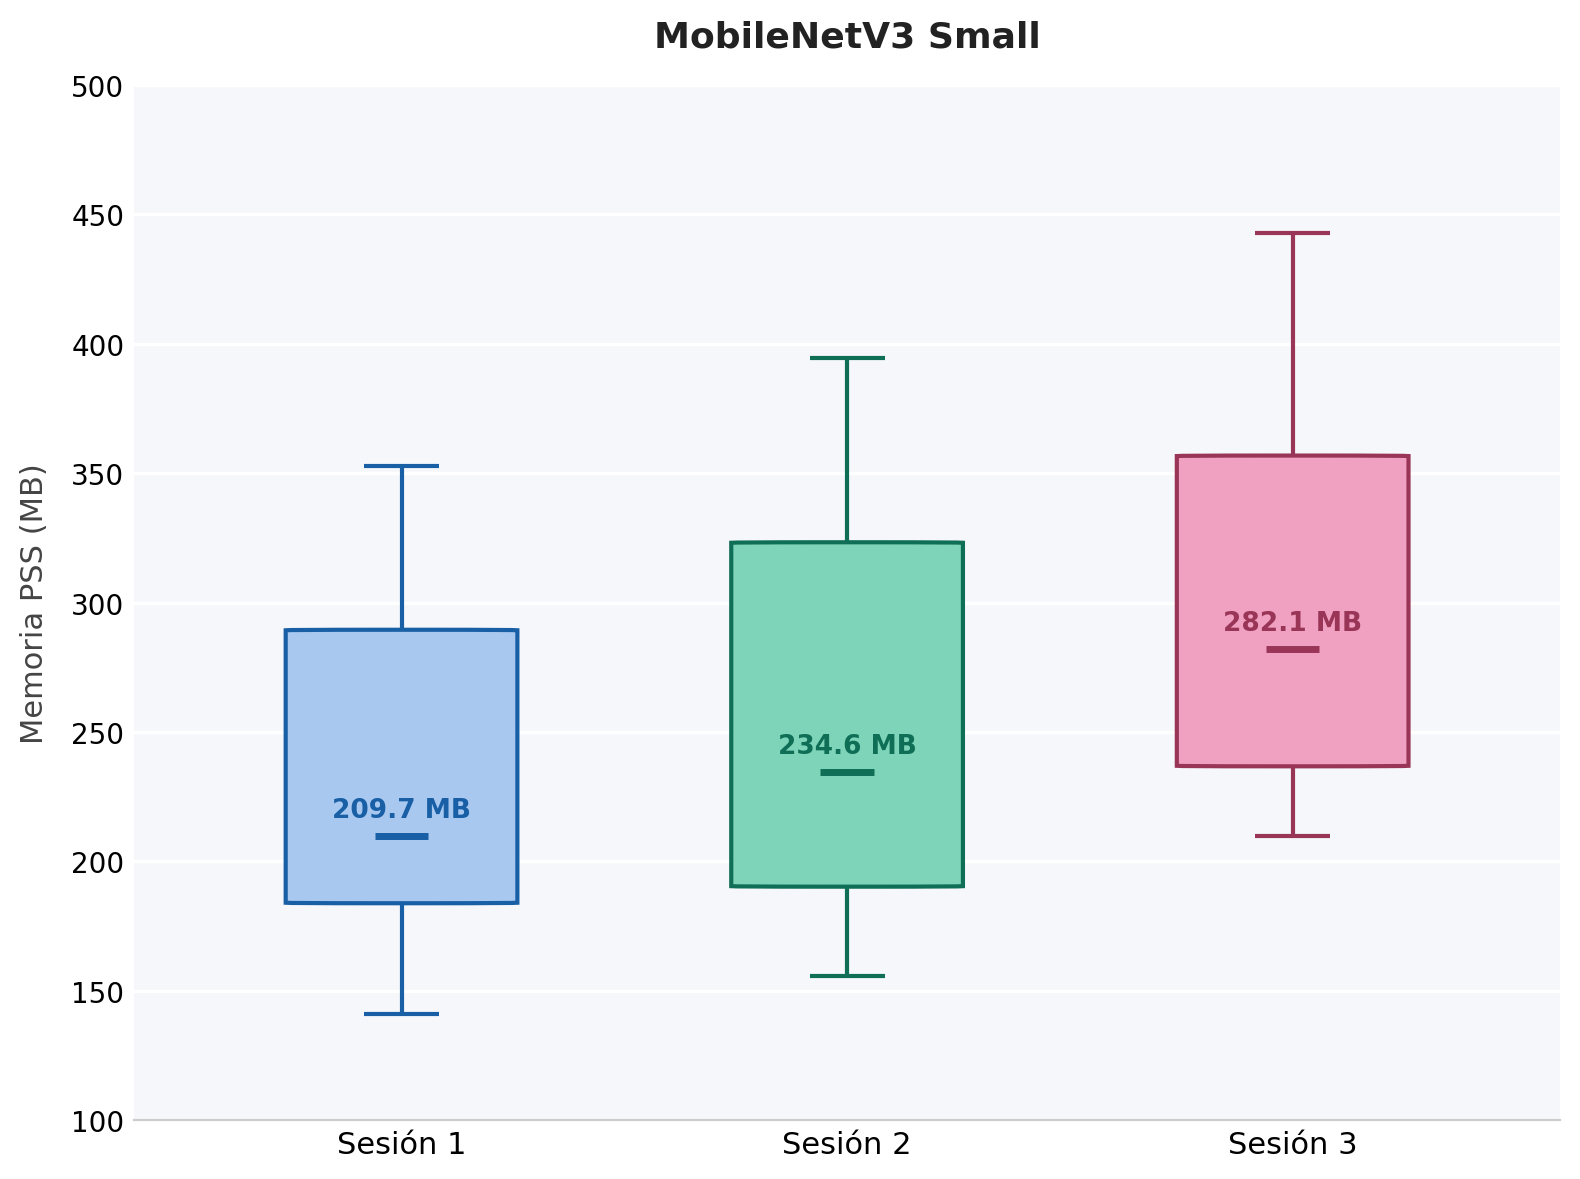
\includegraphics[width=\textwidth]{images/PSS_MobileNetV3Small_MotoG.png}
    \end{minipage}
    \hfill
    \begin{minipage}{0.49\textwidth}
        \centering
        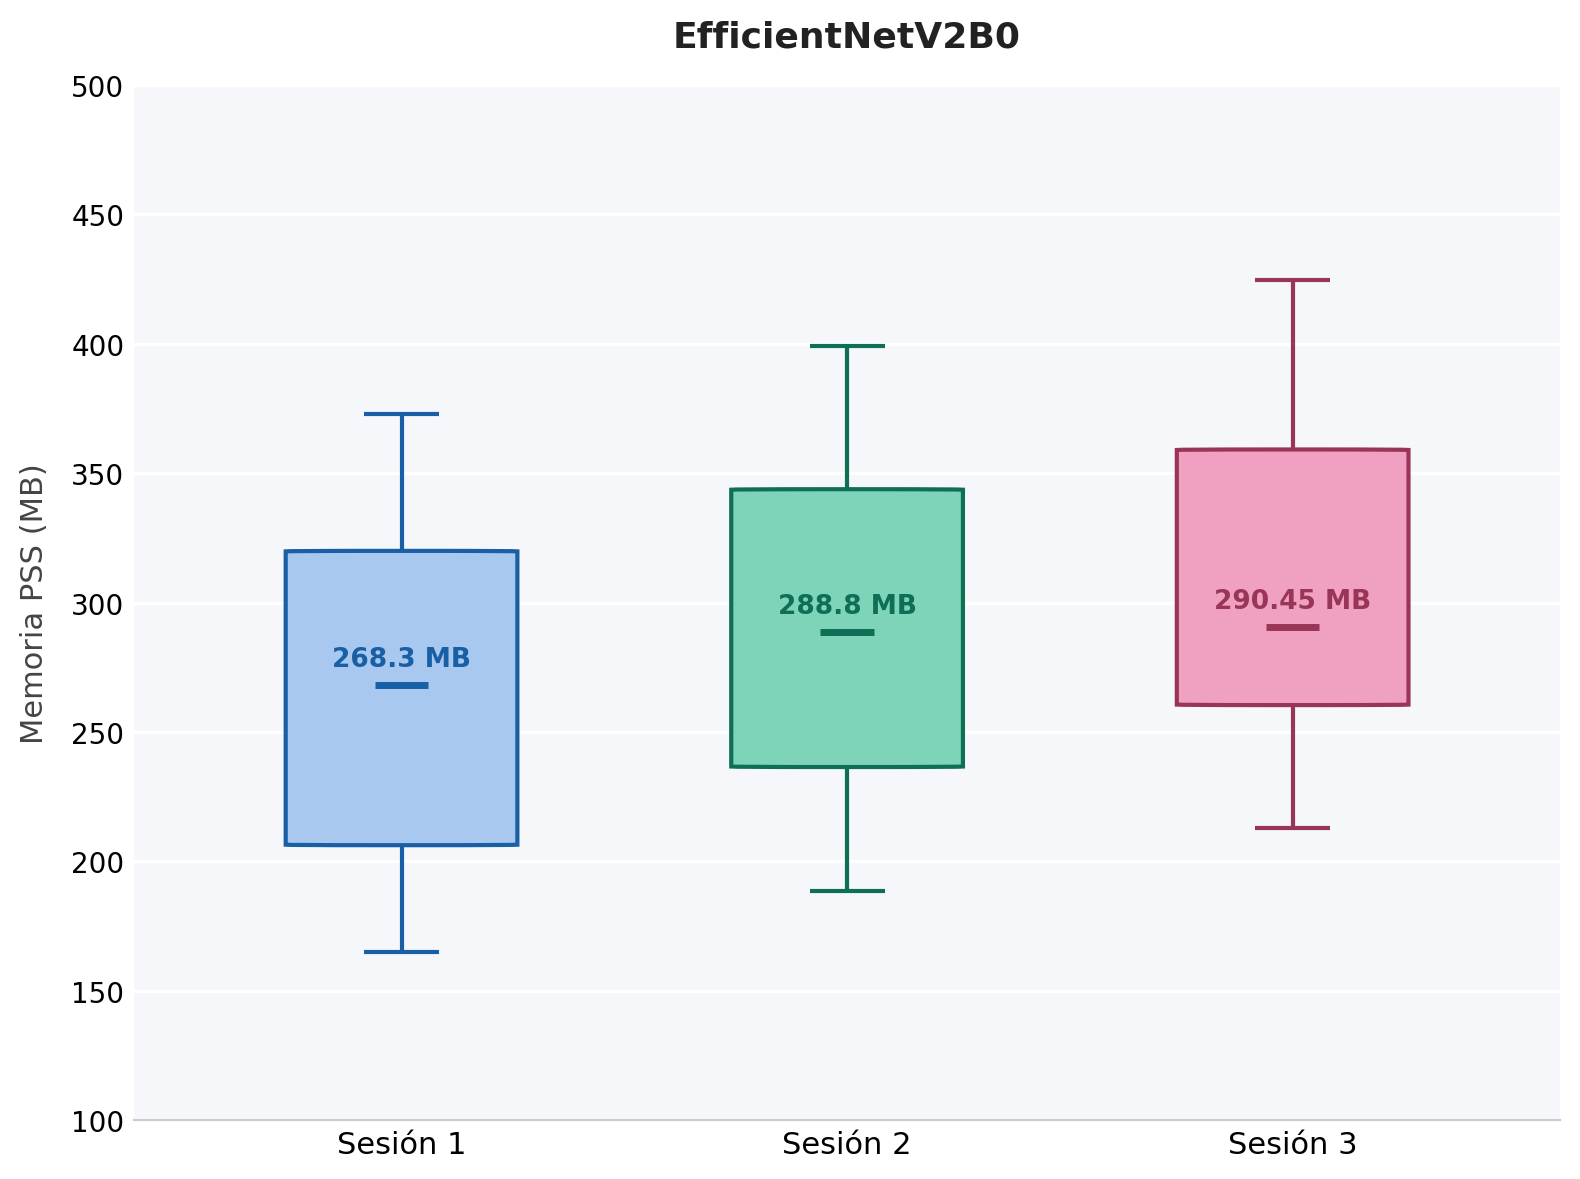
\includegraphics[width=\textwidth]{images/PSS_EfficientNetV2B0_MotoG.png}
    \end{minipage}
    \caption{Distribución de memoria PSS en Moto G30 para MobileNetV3 Small y EfficientNetV2B0.\label{fig:pss_motog_models}}
\end{figure}

La figura \ref{fig:pss_samsung_models} presenta la misma medición en el Samsung Galaxy S23, permitiendo comparar el comportamiento de
memoria de ambos modelos en un dispositivo con mayores recursos de hardware.

\begin{figure}[H]
    \centering
    \begin{minipage}{0.49\textwidth}
        \centering
        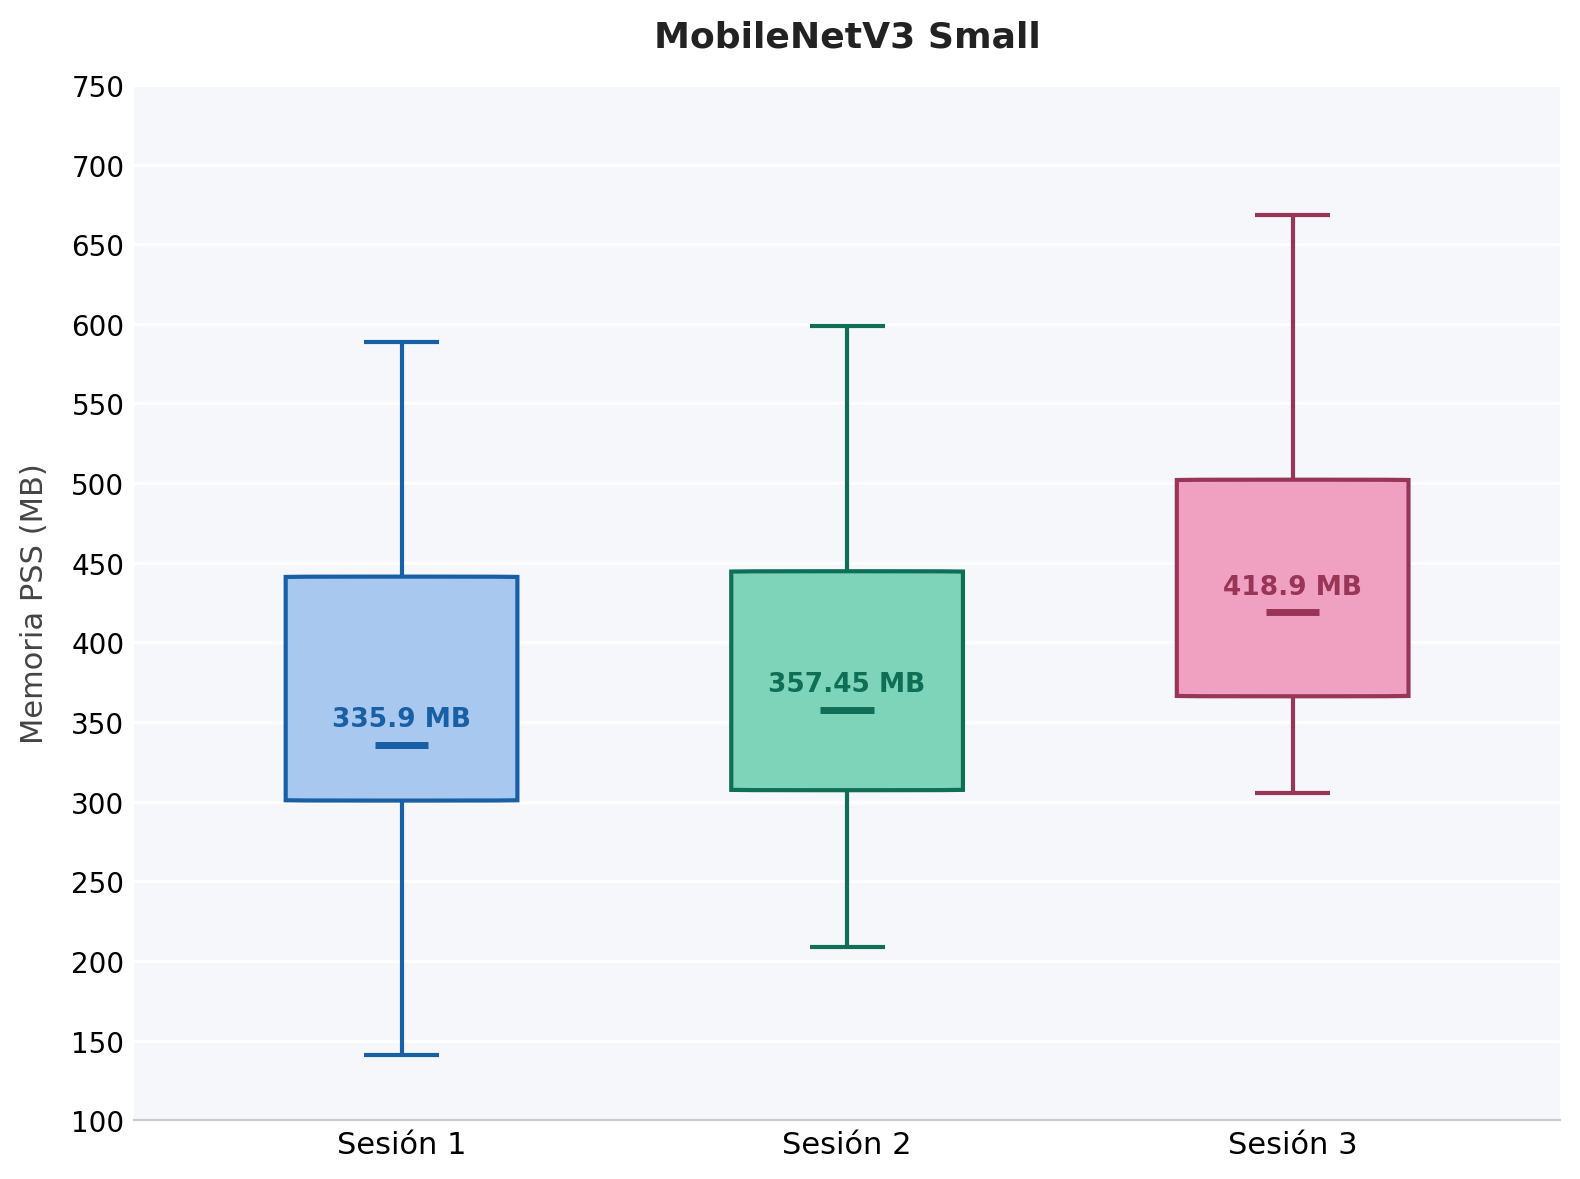
\includegraphics[width=\textwidth]{images/PSS_MobileNetV3Small_SamsungS23.png}
    \end{minipage}
    \hfill
    \begin{minipage}{0.49\textwidth}
        \centering
        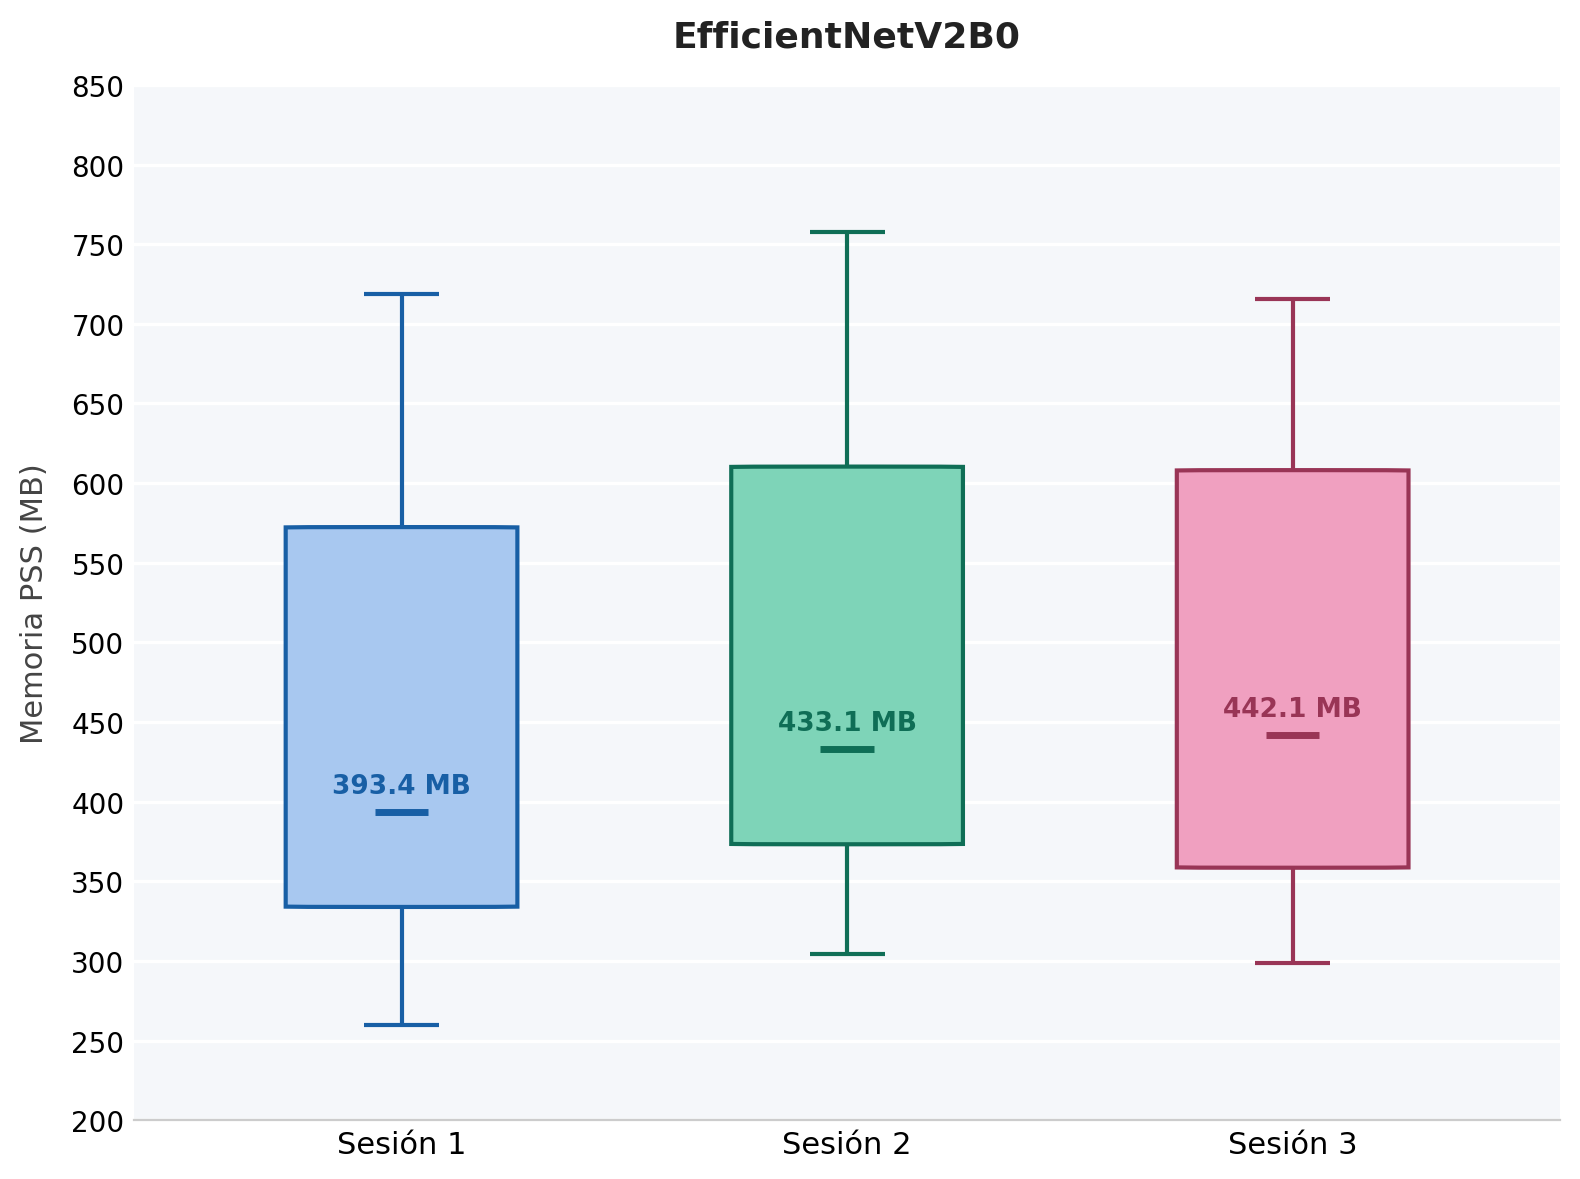
\includegraphics[width=\textwidth]{images/PSS_EfficientNetV2B0_SamsungS23.png}
    \end{minipage}
    \caption{Distribución de memoria PSS en Samsung Galaxy S23 para MobileNetV3 Small y EfficientNetV2B0.\label{fig:pss_samsung_models}}
\end{figure}


El consumo de memoria PSS en ambos dispositivos tiene una tendecia creciente durante la ejecucion de los modelos en las 3 sesiones de prueba, aunque con una variabilidad considerable. 
En el Moto G30, MobileNetV3 Small presentó un consumo promedio general de ~263 MB, mientras que EfficientNetV2B0 tuvo un consumo promedio de ~285 MB. En el Samsung
Galaxy S23, MobileNetV3 Small mostró un consumo promedio de ~394 MB, mientras que EfficientNetV2B0 registró un consumo promedio de ~466 MB. En ambos dispositivos, EfficientNetV2B0 presentó un 
consumo de memoria mayor que MobileNetV3 Small, lo cual es consistente con su arquitectura más compleja y su mayor número de parámetros.
El crecimiento progresivo de PSS a lo largo de la sesión indica acumulación de buffers intermedios. No se registraron OOM ni crashes en ninguna sesión.
Ademas se observa que el dispositivo Samsung al tener más RAM disponible (8 GB vs. 4 GB) el sistema operativo permite que la app ocupe más memoria sin presión.
Esto explica valores de PSS mayores en valor absoluto respecto al Moto G.


\subsection{Consumo de batería}

\subsection{Temperatura del dispositivo}

\subsection{Coherencia botánica}

En el dispositivo Moto G30, ambos modelos fueron consistentes es su clasificacion y confianza durante las tres sesiones de prueba, obteniendo el mismo 
diagnóstico para cada imagen evaluada. 


\chapter{Conclusiones}
Un conjunto de datos de calidad es el requisito fundamental para establecer la base de un modelo de aprendizaje profundo (deep learning), 
ya que el rendimiento de dicho modelo depende en gran medida de la calidad, cantidad y relevancia del conjunto de datos. Por lo tanto,
el primer paso crucial de cualquier aprendizaje profundo comienza con la adquisición de imágenes.

El proceso de adquisición de datos no solo implica capturar la información, sino asegurar que esta sea representativa del entorno real donde 
se desplegará el modelo, lo cual es el primer filtro para evitar sesgos y errores en etapas posteriores de entrenamiento \cite{Khan2023}.

\bibliographystyle{plain} % Estilo de la bibliografía (ej: plain, unsrt, alpha)
\bibliography{bibliografia} % El nombre de tu archivo .bib (sin extensión)
\end{document}
